\documentclass[11pt]{article}
\usepackage{amsmath,amssymb,float,amsfonts,enumitem,tcolorbox}
\usepackage{enumitem}
\usepackage[margin=0.7in]{geometry}

\usepackage{graphicx}


\title{Project 2 Cloud Data}
\author {Caiyi Deng 3033303379, Winnie Gao 3031884025}


\usepackage{Sweave}
\begin{document}
\Sconcordance{concordance:new_report.tex:new_report.Rnw:%
1 7 1 1 7 5 1 1 0 151 1}


\maketitle

\section{Data Collection and Exploration}

\vspace{0.2cm}
\textbf{a. Summary of Paper}

Climate changes has been a popular topic in scientific research. Particularly, the warming Arctic is one of the biggest stories in our times. Global climate models predict that the increasing atmospheric carbon dioxide levels is strongly related to the increasing surface air temperatures in the Arctic, where cloud plays an important role in producing more atmospheric carbon dioxide. In this paper, scientists use the Multiangle Imaging SpectroRadiometer (MISR) imagery to perform a cloud detection to ascertain whether cloud can potentially lead to further warming in the Arctic.

MISR collects a massive amount of data from its nine cameras viewing at a different angel in four spectral. It covers the daylight side of the Earth from the Arctic down to Antarctica in 45 minutes and completes all paths in 16 days of a cycle. Each path is subdivided into blocks, with the block numbers increasing from the North Pole to South Pole, and each complete trip of MISR around the Earth is counted as a unique orbit. However, due to the transmission channel constraints, only the red radiances and all channels from the nadir camera are transmitted at full 275m * 275m resolution. The remaining blue, green and near-infrared radiances from the non-nadir cameras are aggregated to a lower resolution before transmission. 

Scientists utilizes correlations in brightness among multiple MISR views of the same scene under cloud-free conditions to model the surface. This new algorithm, enhances linear correlation matching (ELCM), is based on thresholding three features: the correlation (CORR) of MISR images, the standard deviation (SD\_An) of the MISR nadir camera pixel values, and a normalized difference angular index (NDAI) to create labels for classification. Then, the resulting labels are used in the second algorithm, ELCM-QDA, to produce more informative probability prediction. 

The results suggest that the ELCM algorithm based on the three features outperform those existing algorithms based only on the radiation measurement, where it provides better spatial coverage for cloud detection in the Arctic. Moreover, the ELCM algorithm combines classification and clustering framework to fit the MISR data processing, which help improve the computational speed online effectively. 

This research not only creates a better algorithm to implement cloud detection but also encourages further study on the changing cloud properties to the warming Arctic. In addition, it demonstrates the significant impact of statistics in successfully solving a modern scientific problem. Statisticians are now directly involved in the data processing and use powerful statistical thinking to help tackle challenges. \par

\vspace{0.3cm}
\mbox{}\\
\textbf{b. Summery of Data}

For image1 data, there are 115229 data points. We calculate \% of pixels for the different classes: 17.77\% classified as cloud, 43.78\% as not cloud and 38.46\% as unlabeled. For image2 data, there are 115110 data points. We calculate \% of pixels for the different classes: 34.11\% classified as cloud, 37.25\% as not cloud and 28.64\% as unlabeled. For image3, there are 115217 data points. We calculate \% of pixels for the different classes: 18.44\% classified as cloud, 29.29\% as not cloud and 52.27\% as unlabeled. After we combined three image data sets, there are 345556 data points. We calculate \% of pixels for the different classes: 23.43\% classified as cloud, 36.78\% as not cloud and 39.79\% as unlabeled. 
In order to view the pattern or trend for the data points, we plot scatter plots and color each data point according to their labels. 


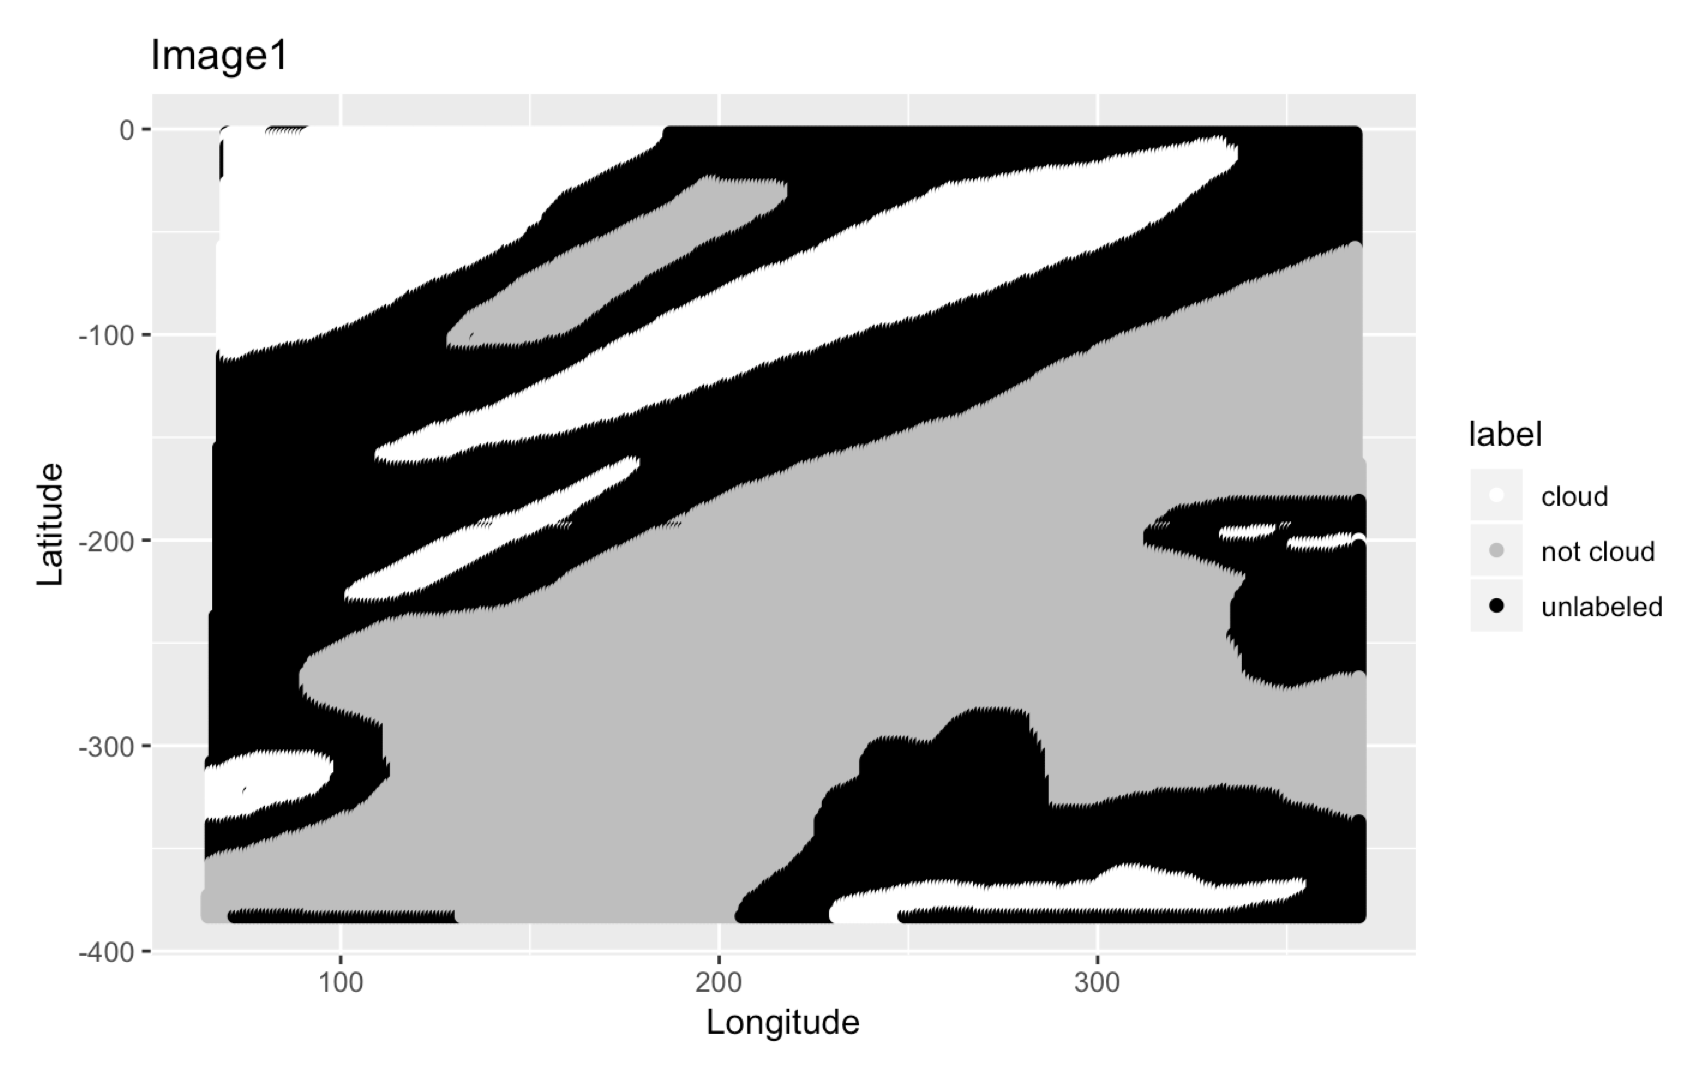
\includegraphics[width = 6cm]{1(b)image1.png}
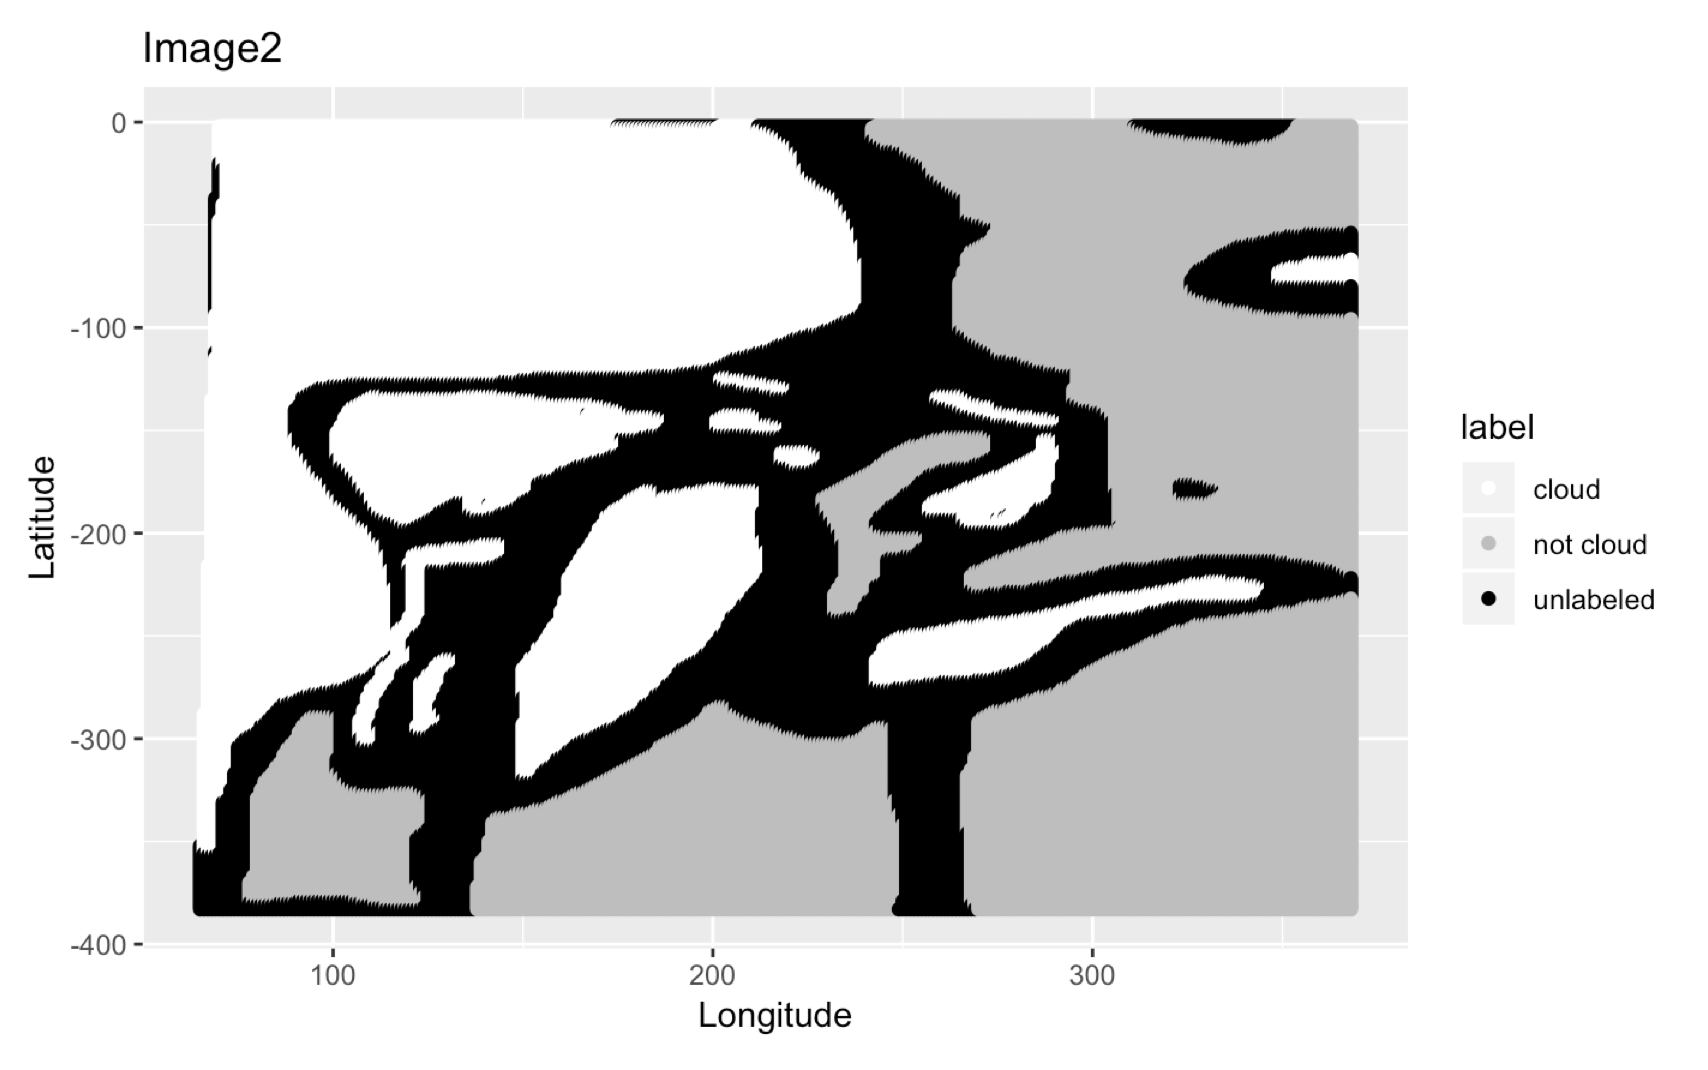
\includegraphics[width = 6cm]{1(b)image2.png}
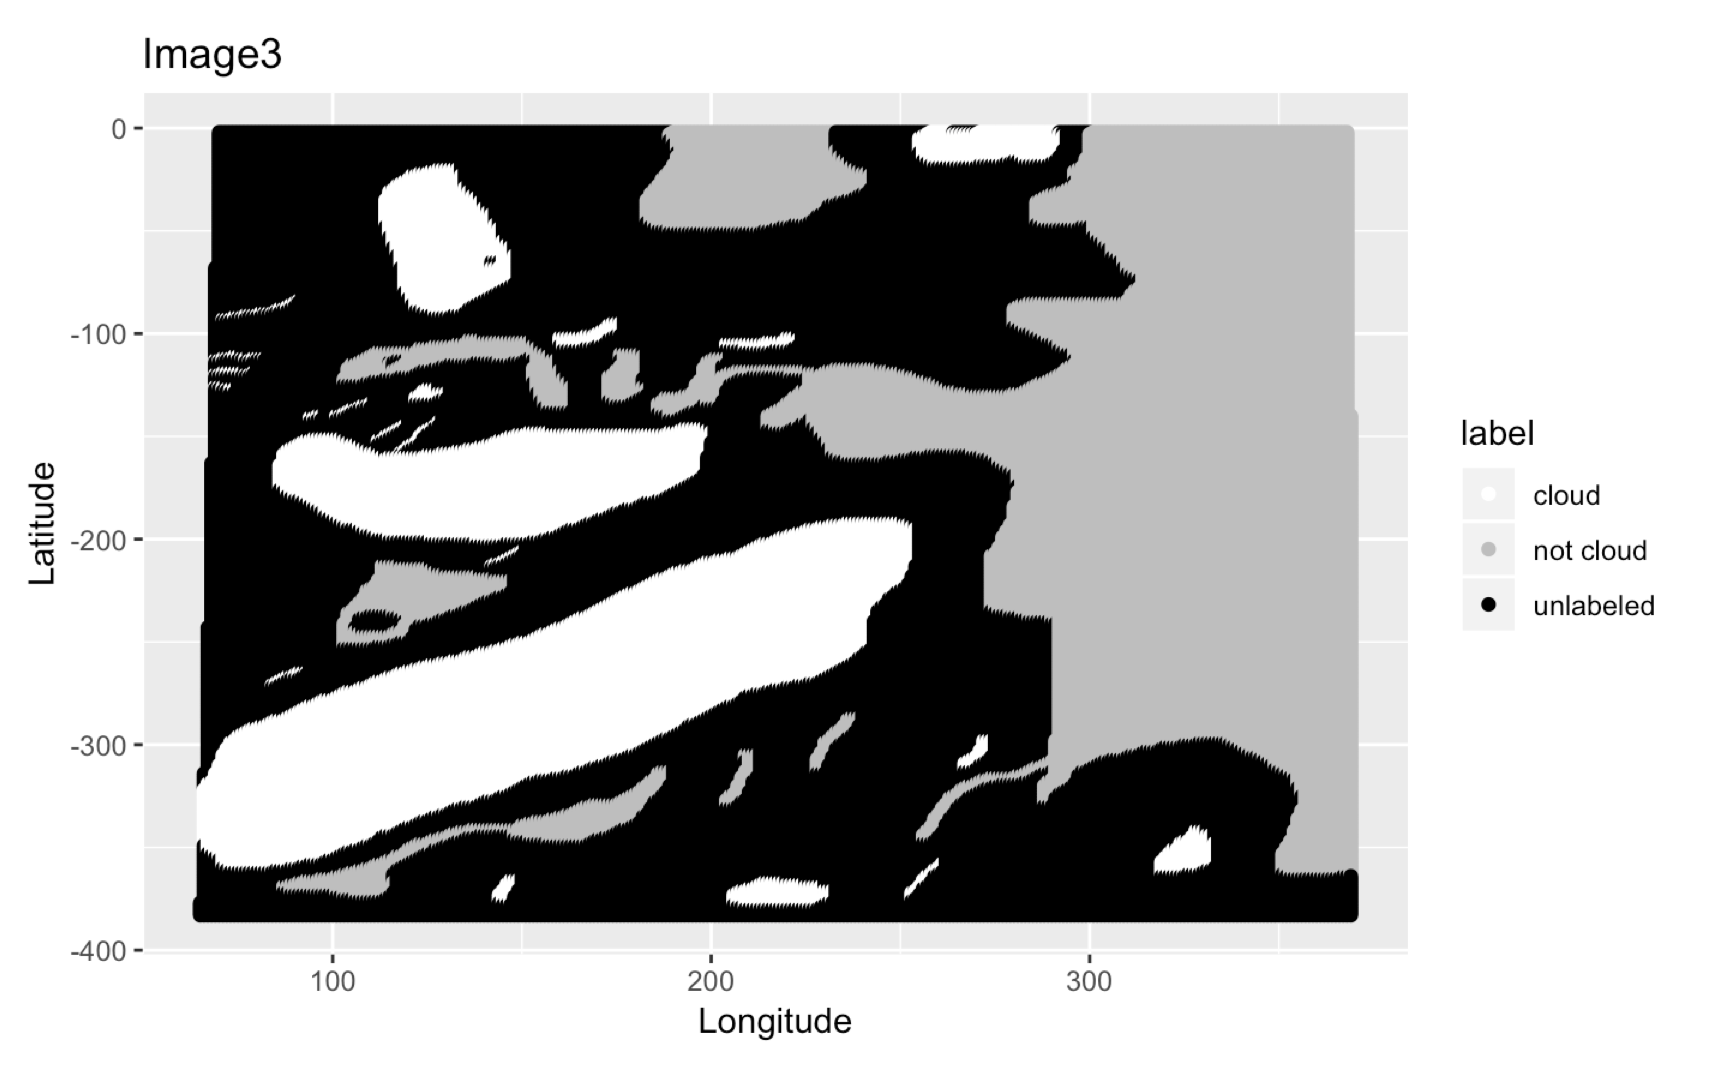
\includegraphics[width = 6cm]{1(b)image3.png}

From the three plots, we can see the pattern that the pixels with same labels are connected to each other, and unmarked pixels stay around those marked as clouds. This pattern contradicts to our assumption that the samples are i.i.d., because the pixels adjcent to pixels marked as clouds are more likely to be marked as clouds.


\vspace{0.3cm}
\mbox{}\\
\textbf{c. EDA}

To further explore our data, we also summarize the pairwise relationship between the features themselves.

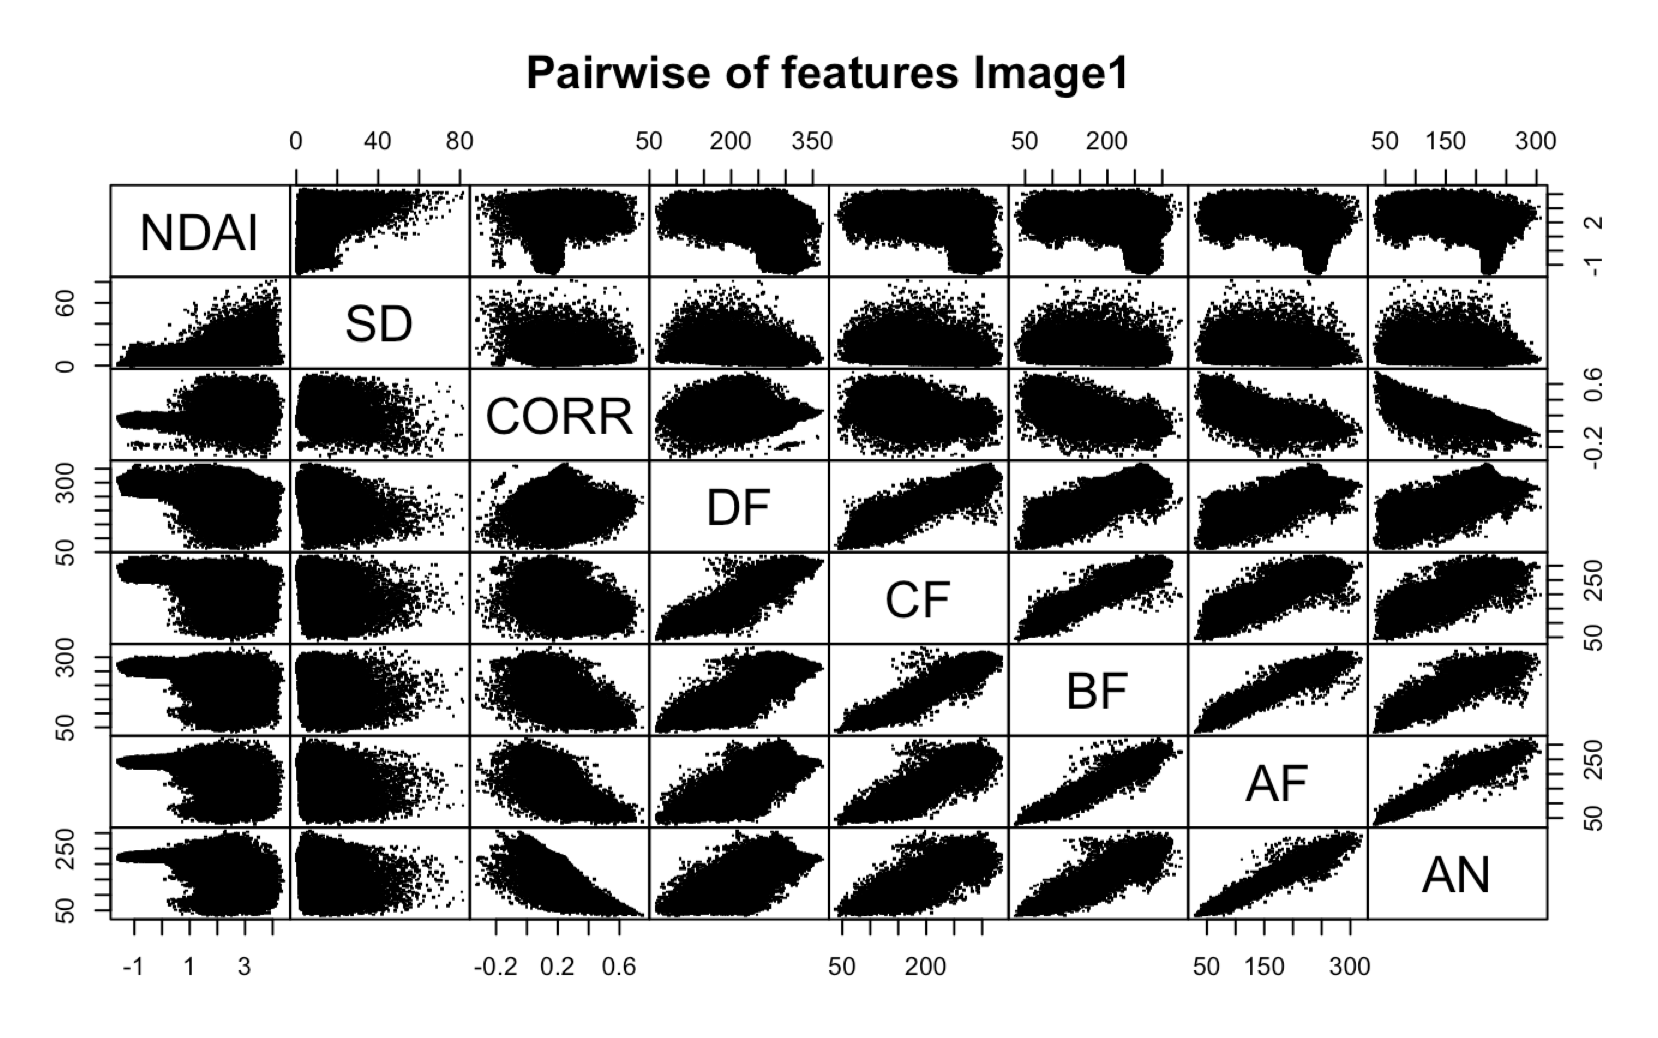
\includegraphics[width = 6cm]{1(c)image1.png}
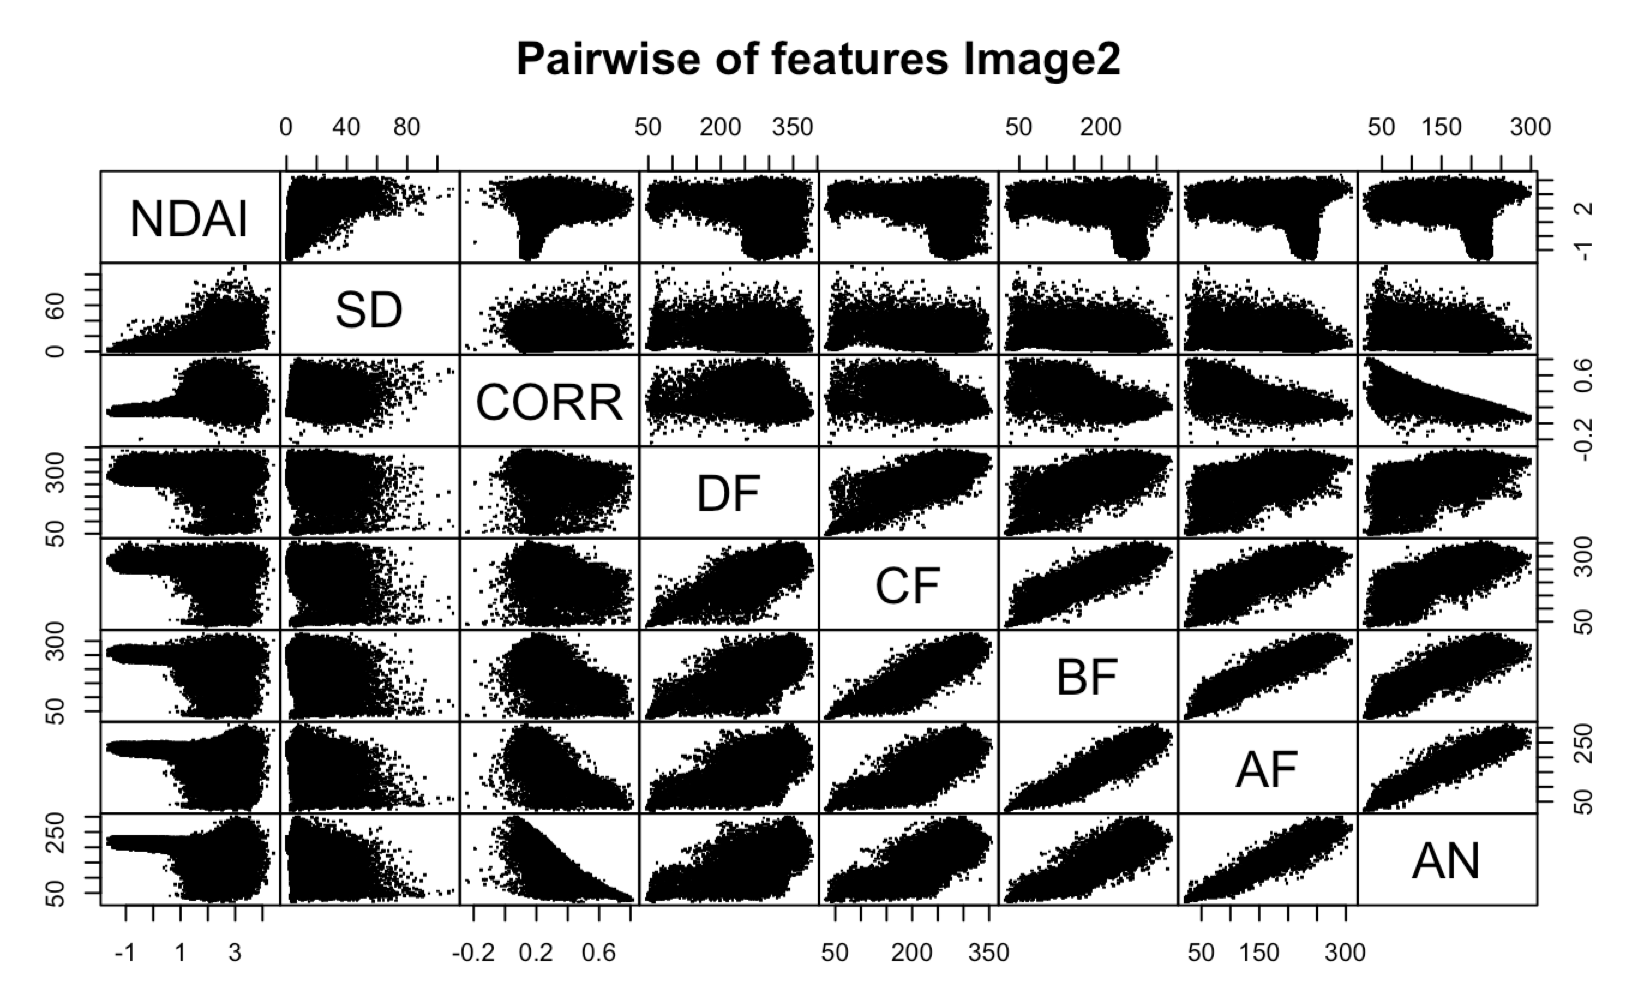
\includegraphics[width = 6cm]{1(c)image2.png}
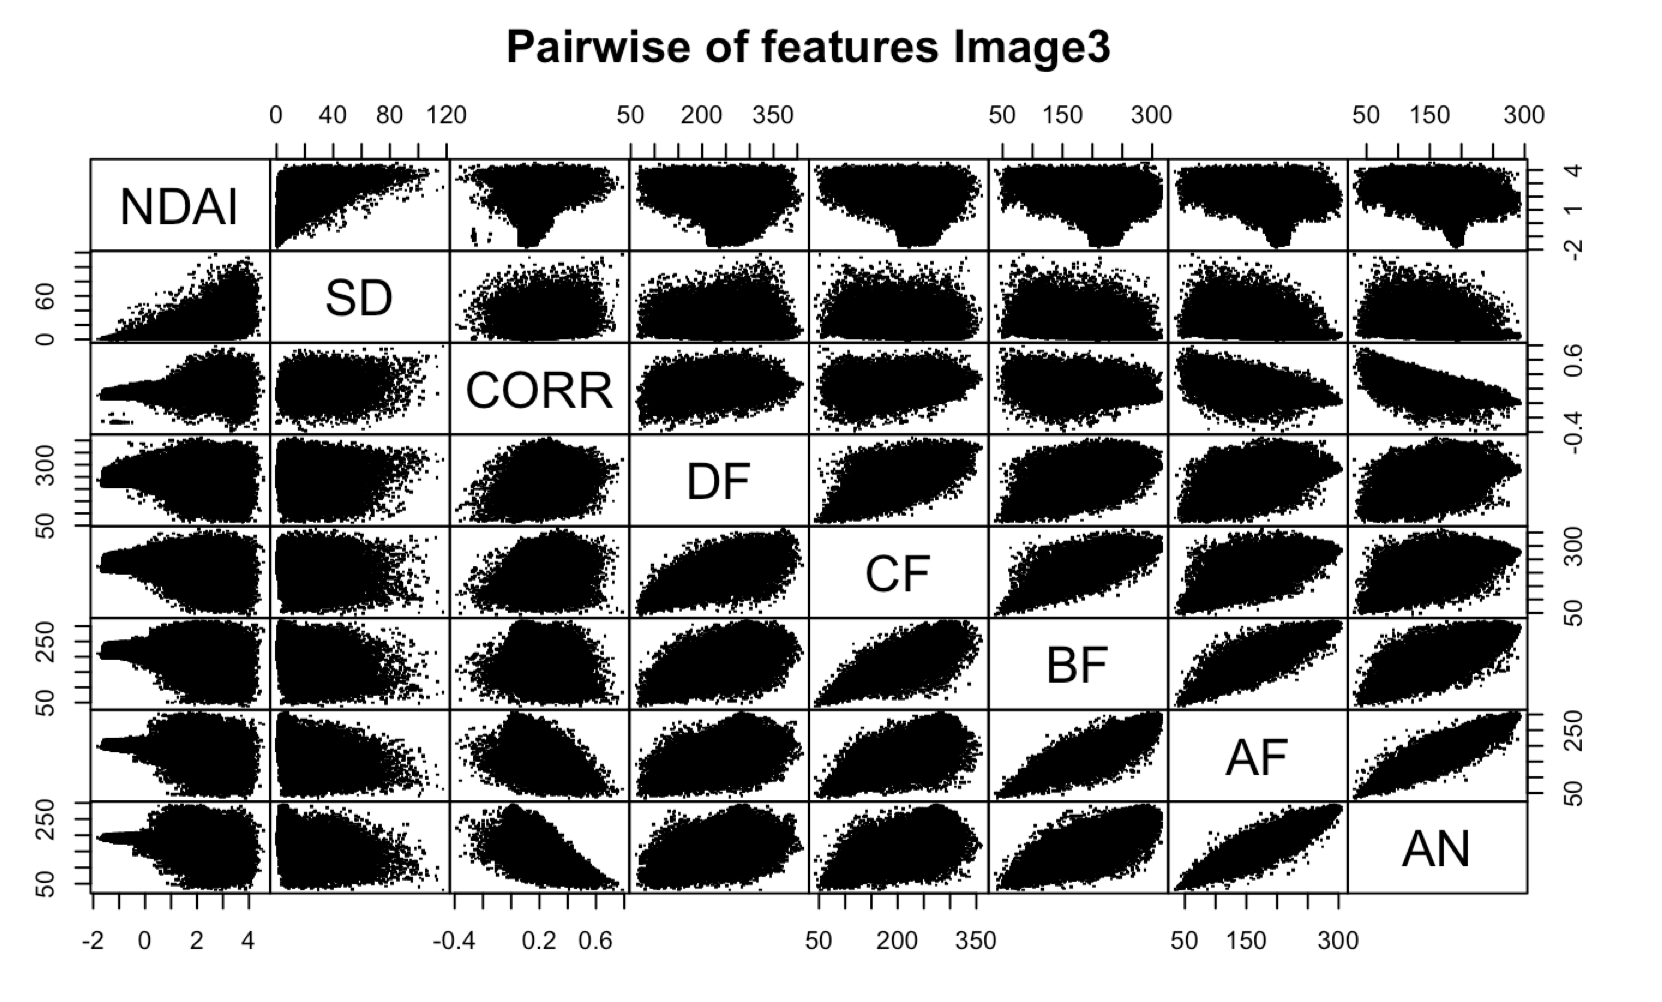
\includegraphics[width = 6cm]{1(c)image3.png}

The three pairwise scatterplots all show that DF, CF, BF, AF and AN shows a linear relationship between each other, especially for AF and AN, AF and BF. However, we observe that data points in the third pairwise scatterplot spread more widely than in the first two pairwise sctterplots. The differences between three graphs can also show that the (linear) relationships decrease over time.

After checking pairwise relationship plots, we study the relationship between each independent featues and their expert labels for each image and all data combined.

(relationship between expert label and NDAI)

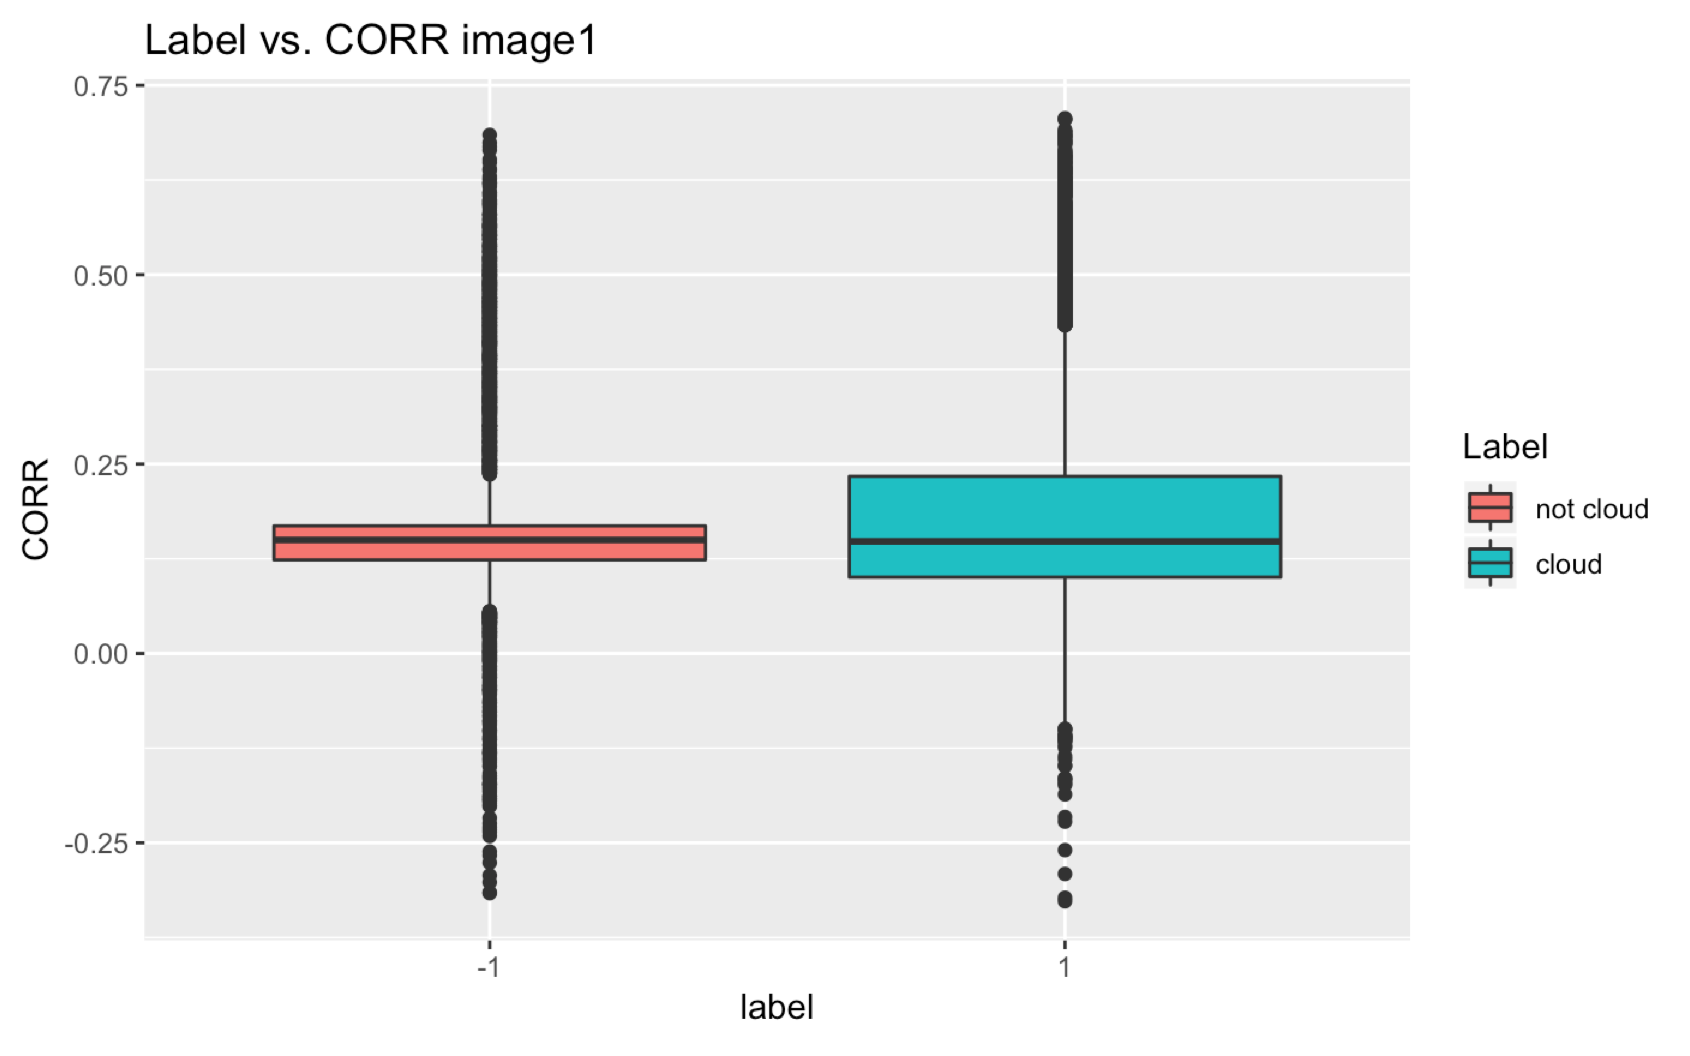
\includegraphics[width = 7.5cm]{1(c)image4.png}
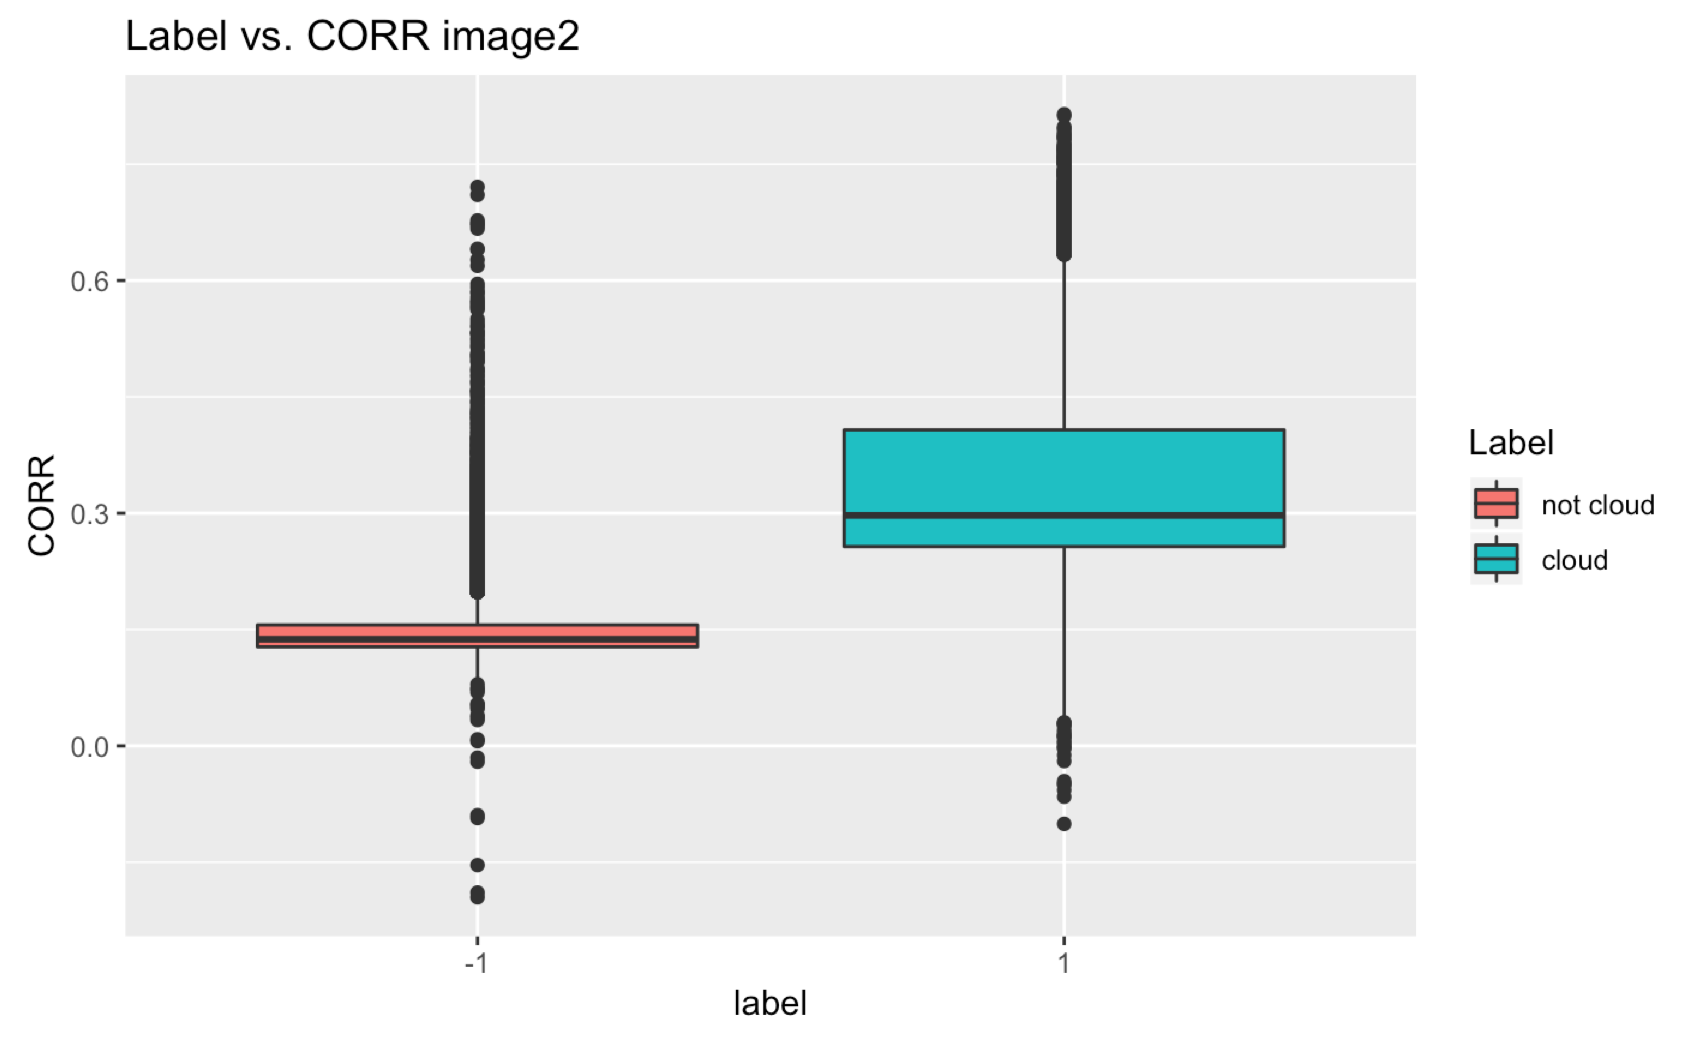
\includegraphics[width = 7.5cm]{1(c)image5.png}

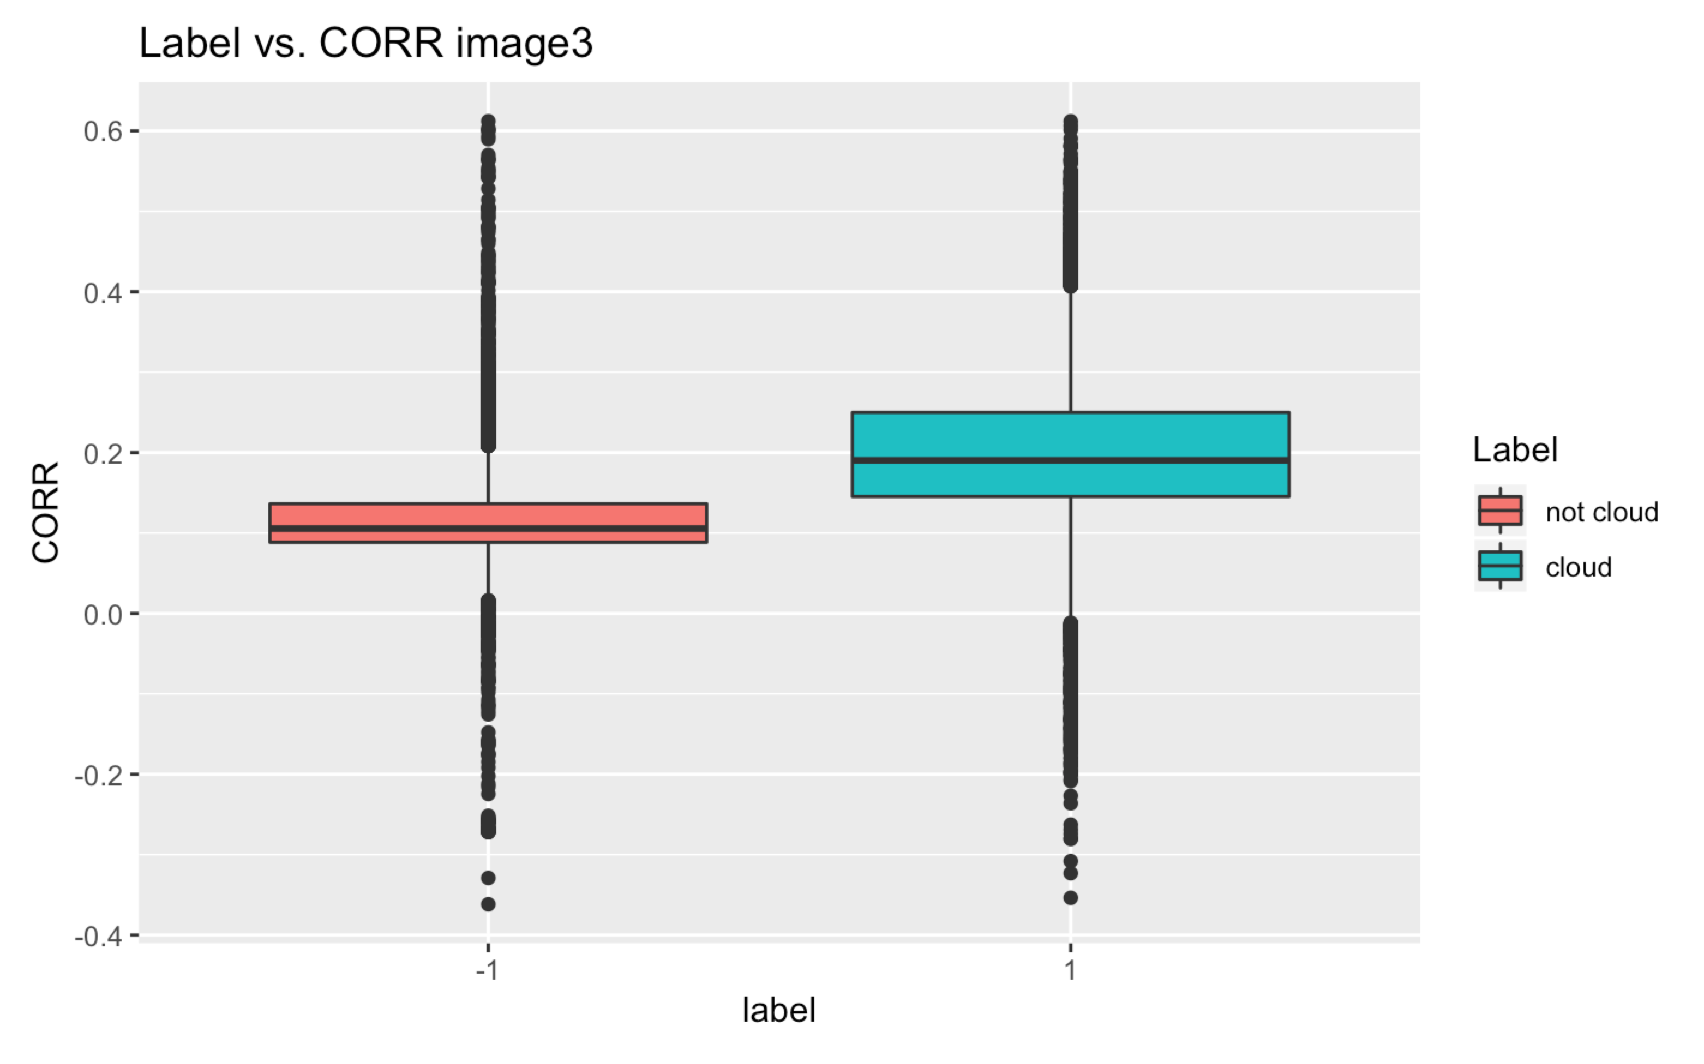
\includegraphics[width = 7.5cm]{1(c)image6.png}
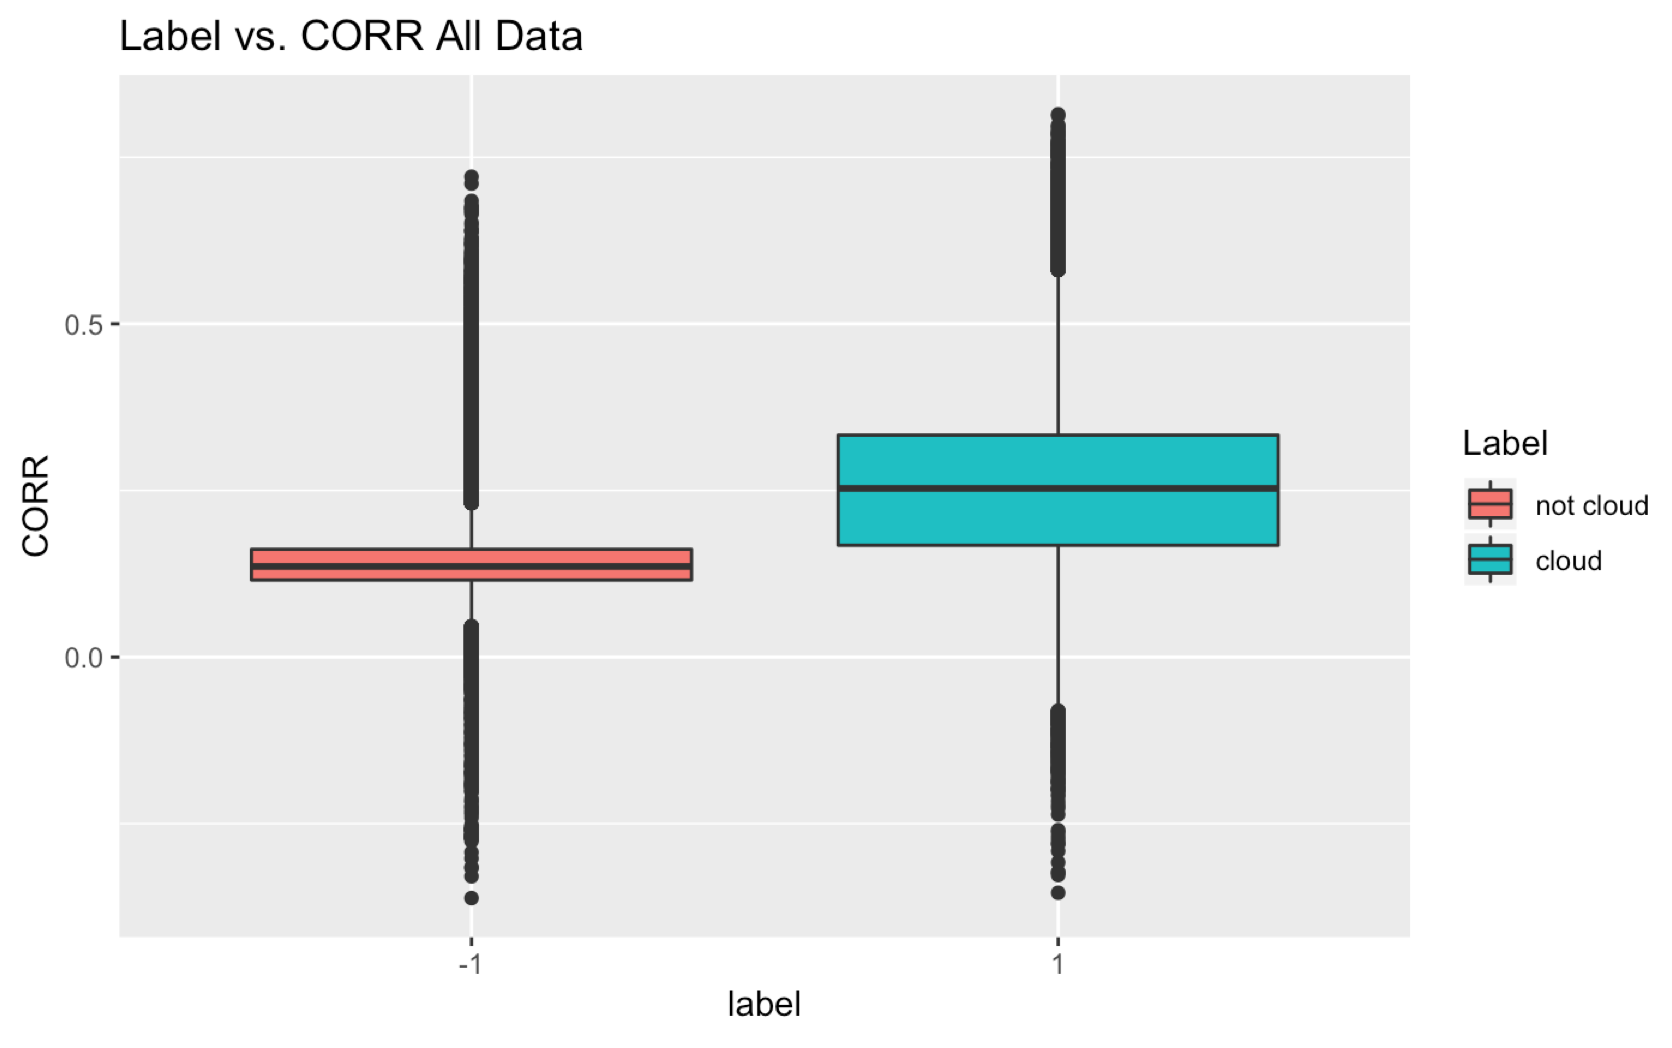
\includegraphics[width = 7.5cm]{1(c)image7.png}

The boxplots for CORR based on different labels show that CORR is on average higher for pixels marked as cloud than as not cloud. CORR also has a higher variance for those marked as cloud.

This conclusion contradicts to the statement in the paper that high correlations over cloud-free areas or low clouds are expected. This is because high correlations for clouds also occur under rare circumstances. More importantly, recklessly declare clear for high CORR pixels and cloudy for low CORR pixels will produce errors due to smoothness of surface terrain and the difference of attitudes of clouds.

Therefore, we should also involve the feature SD to identify surfaces into our investigation. We first plot SD vs. Label independently for each image and all data.

\mbox{}\\
(relationship between expert label and SD)

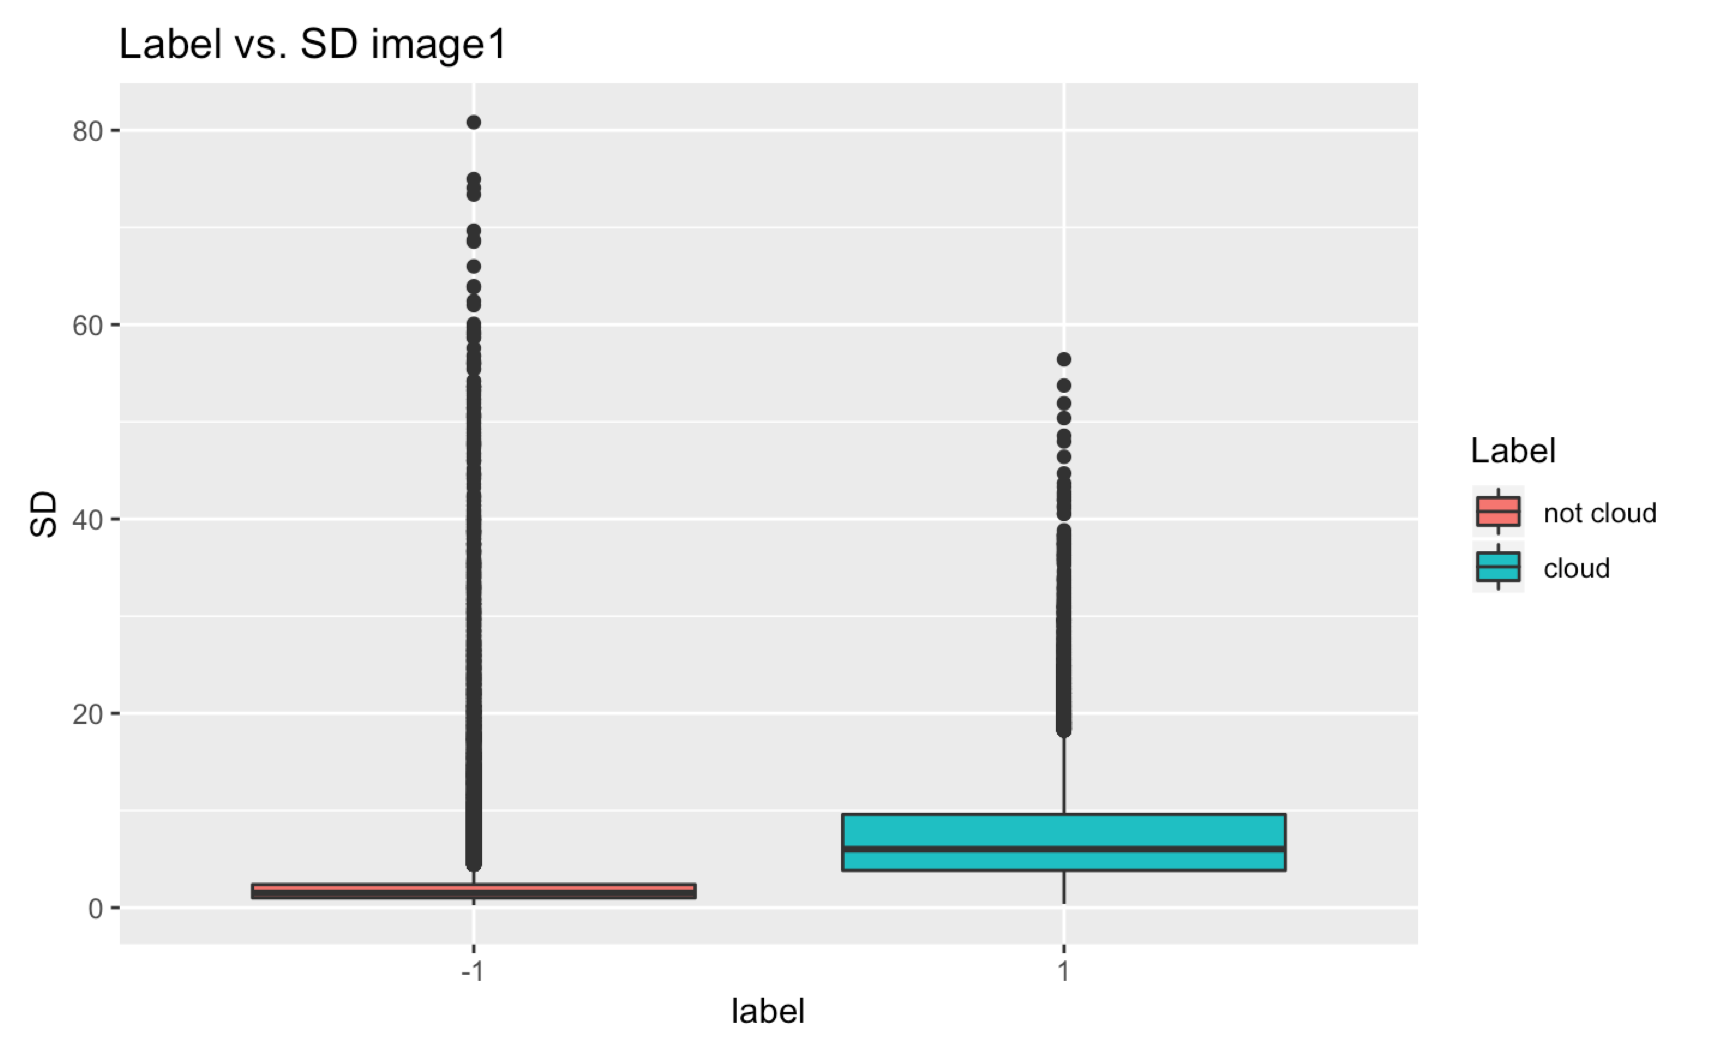
\includegraphics[width = 7.5cm]{1(c)image8.png}
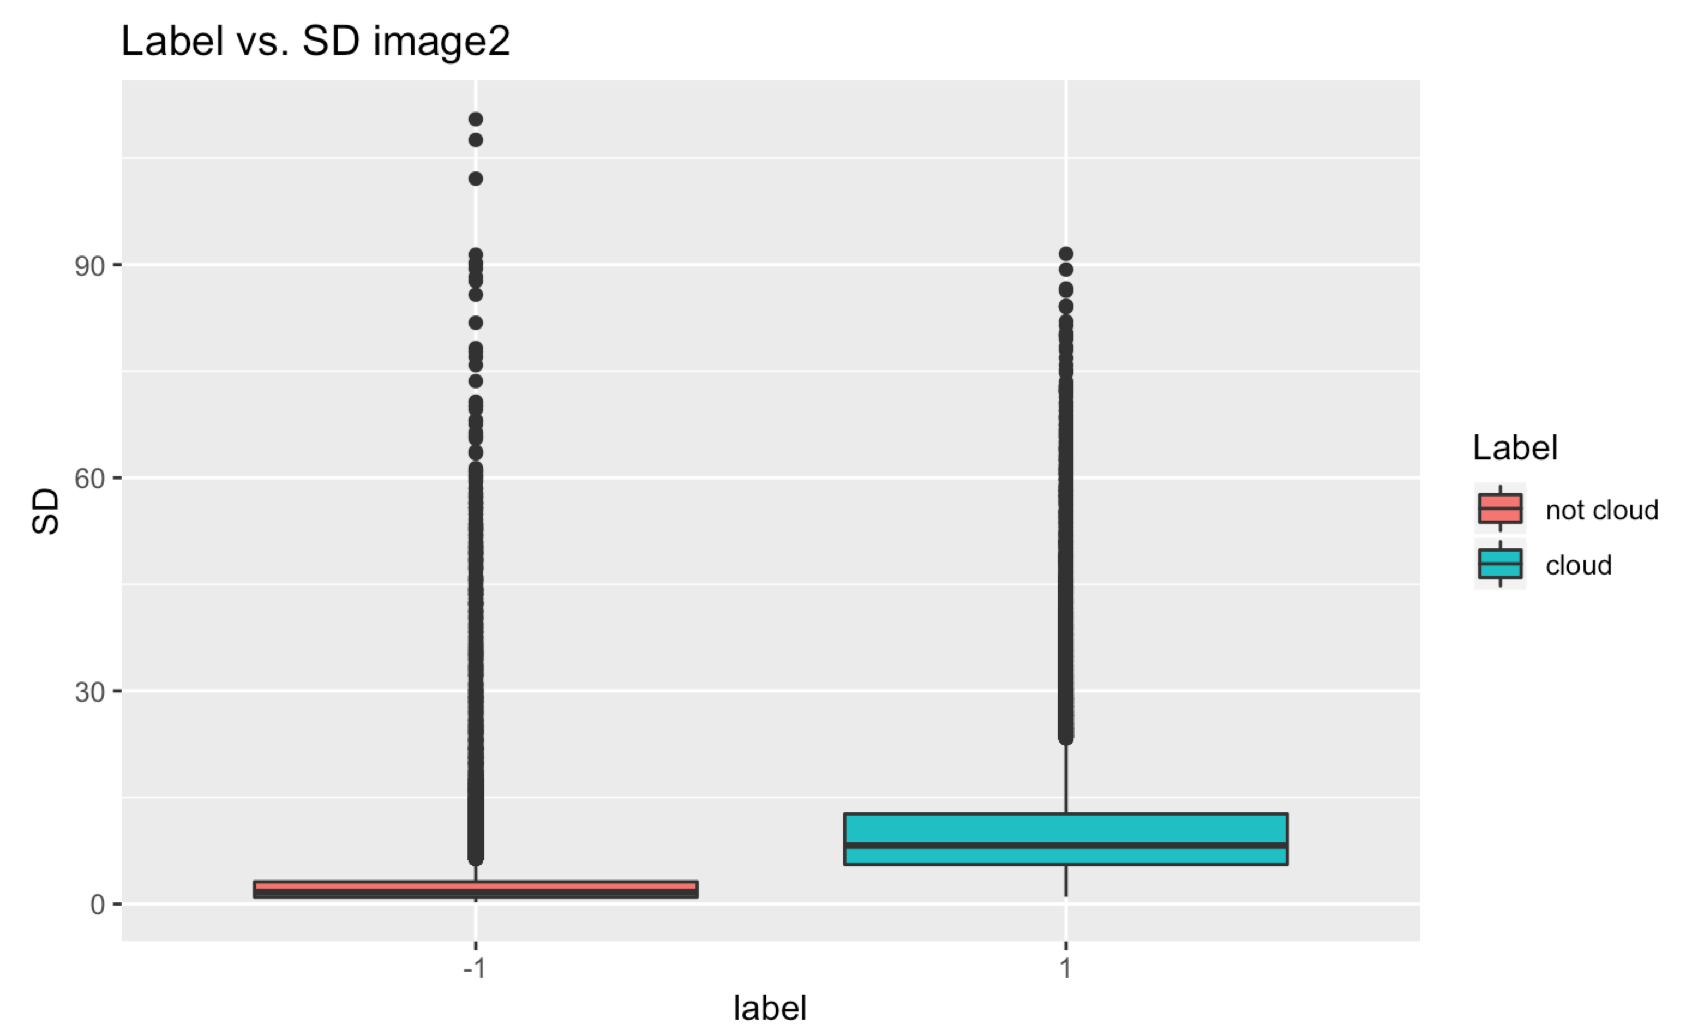
\includegraphics[width = 7.5cm]{1(c)image9.png}

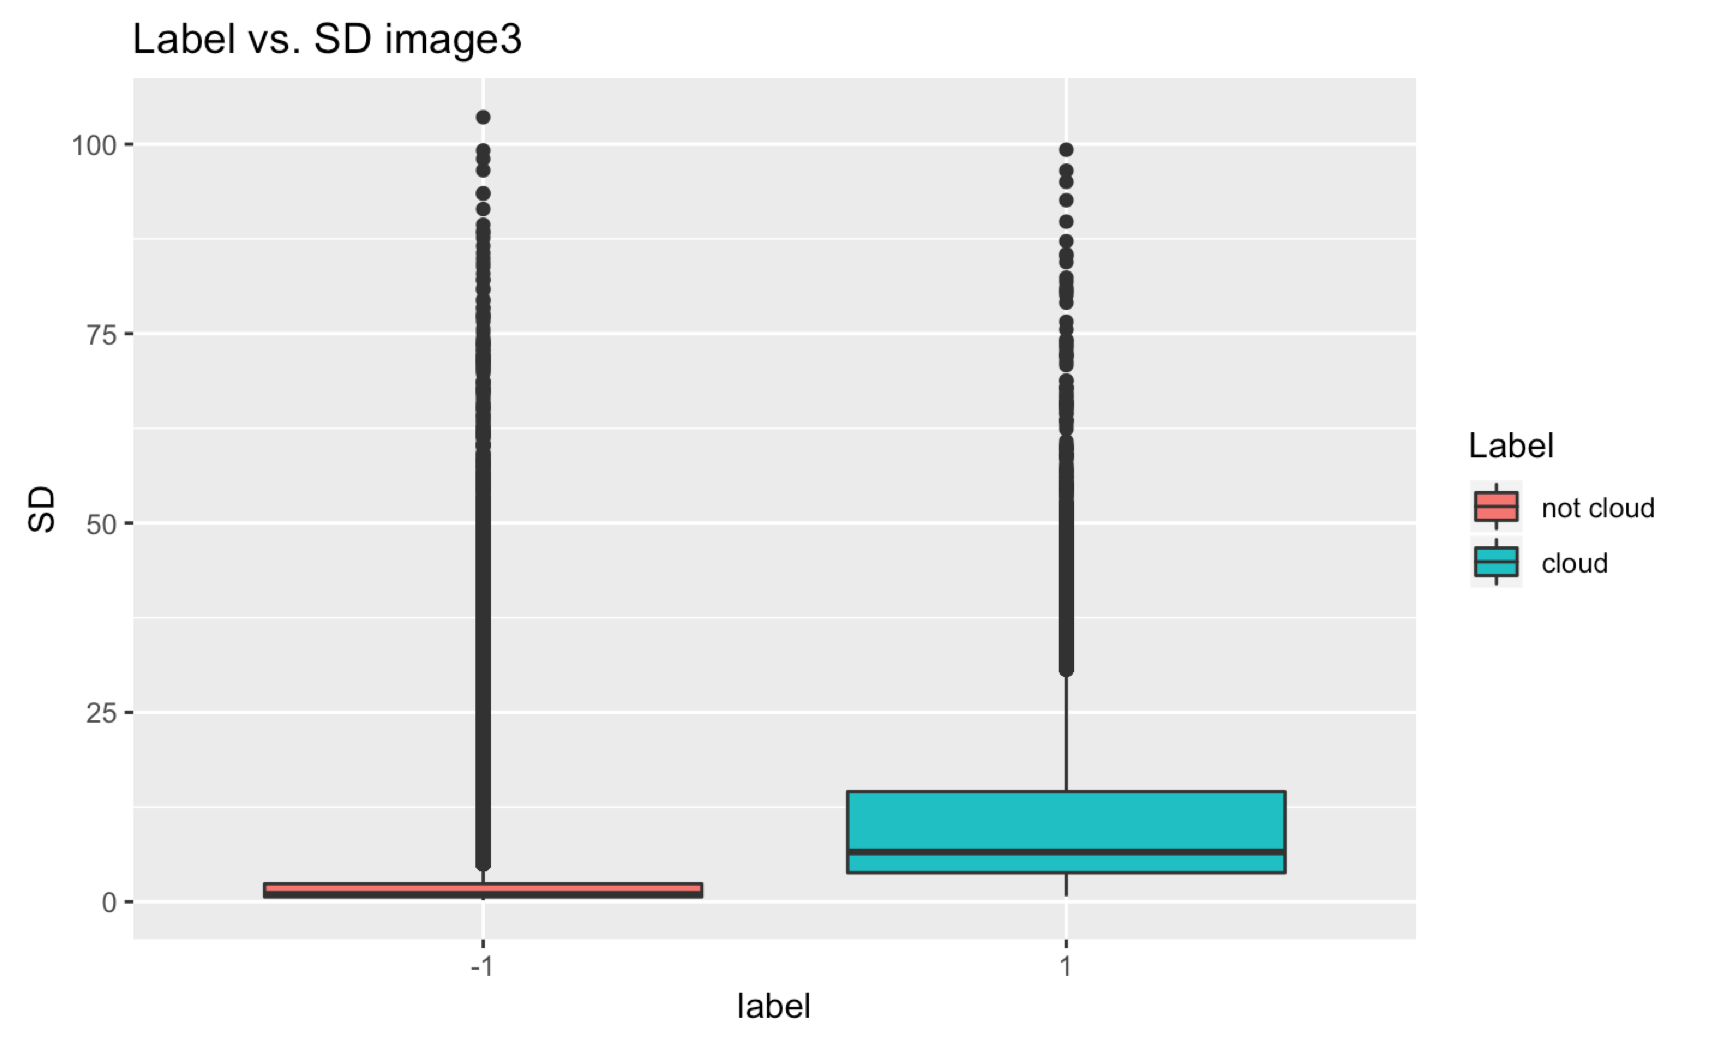
\includegraphics[width = 7.5cm]{1(c)image10.png}
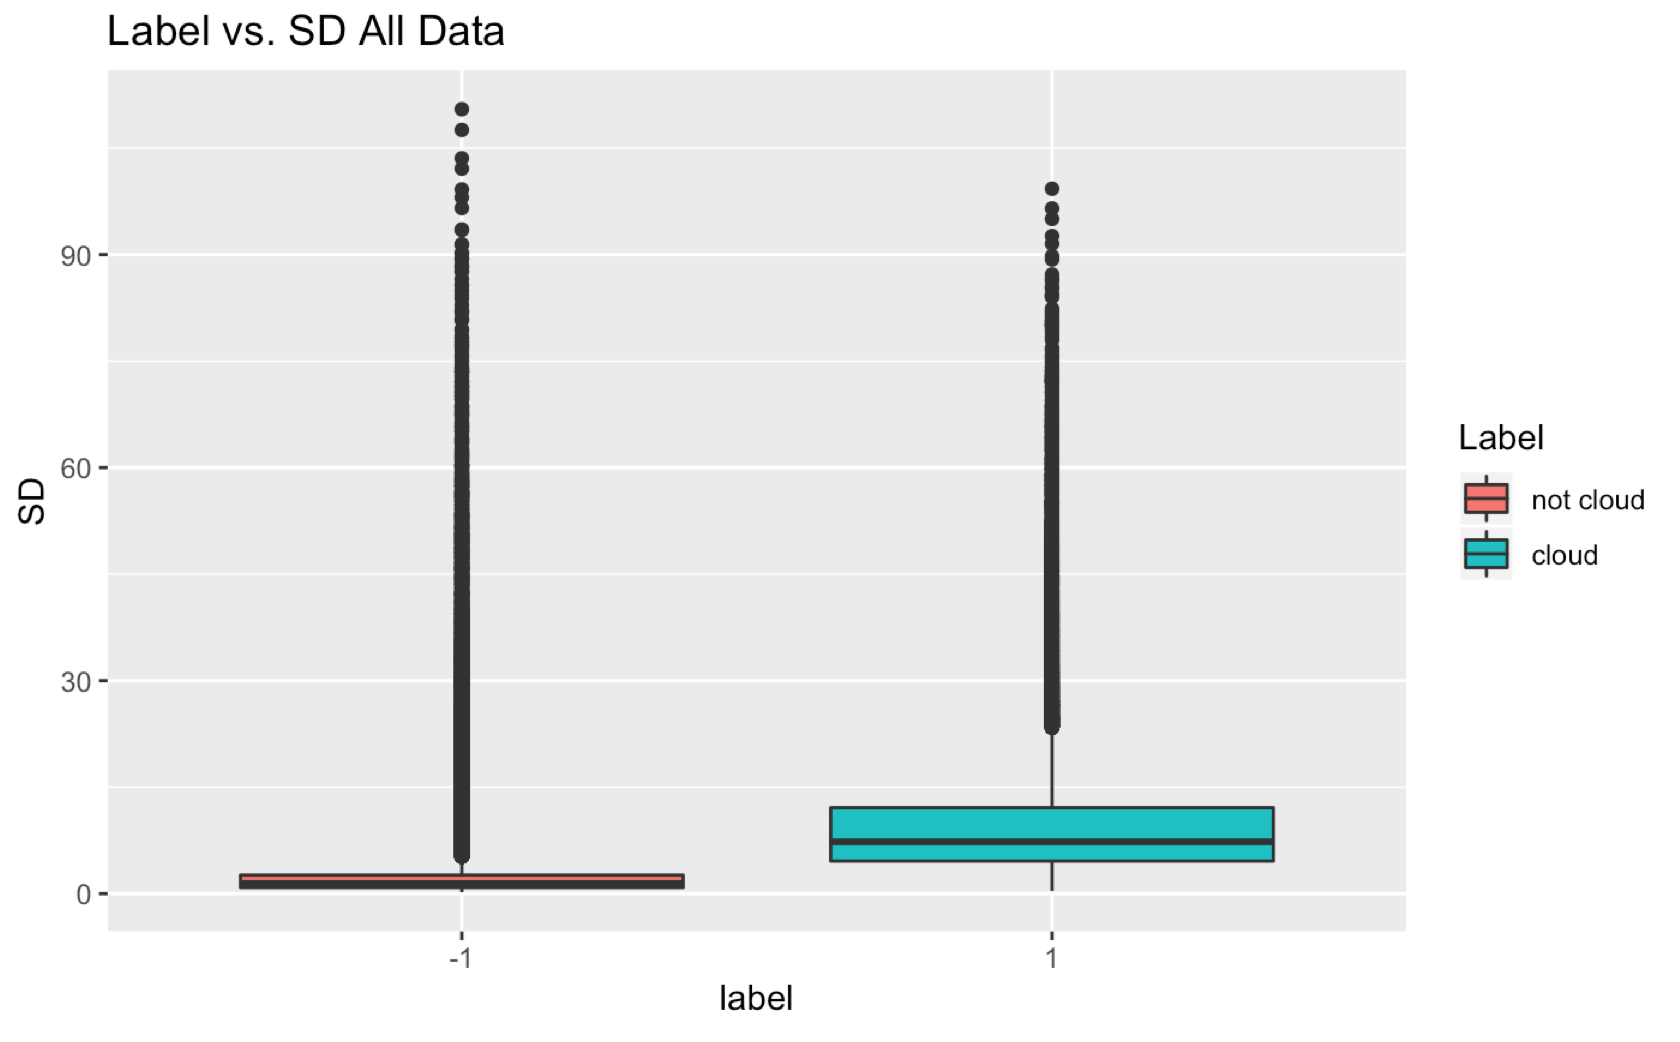
\includegraphics[width = 7.5cm]{1(c)image11.png}

From the boxplots for SD based on different labels, we can clearly see that the SD is higher for cloud pixels than those cloud-free ones. But the cloud-free pixels spread more widely. It can be explained that SD are usually small for radiation emanating from smooth surfaces.

Finally, the thrid feature NDAI relates to the differences for isoreopic level of surface-leaving radiation between low-attitude clouds and snow-coved surfaces.

\mbox{}\\
(relationship between expert label and NDAI)

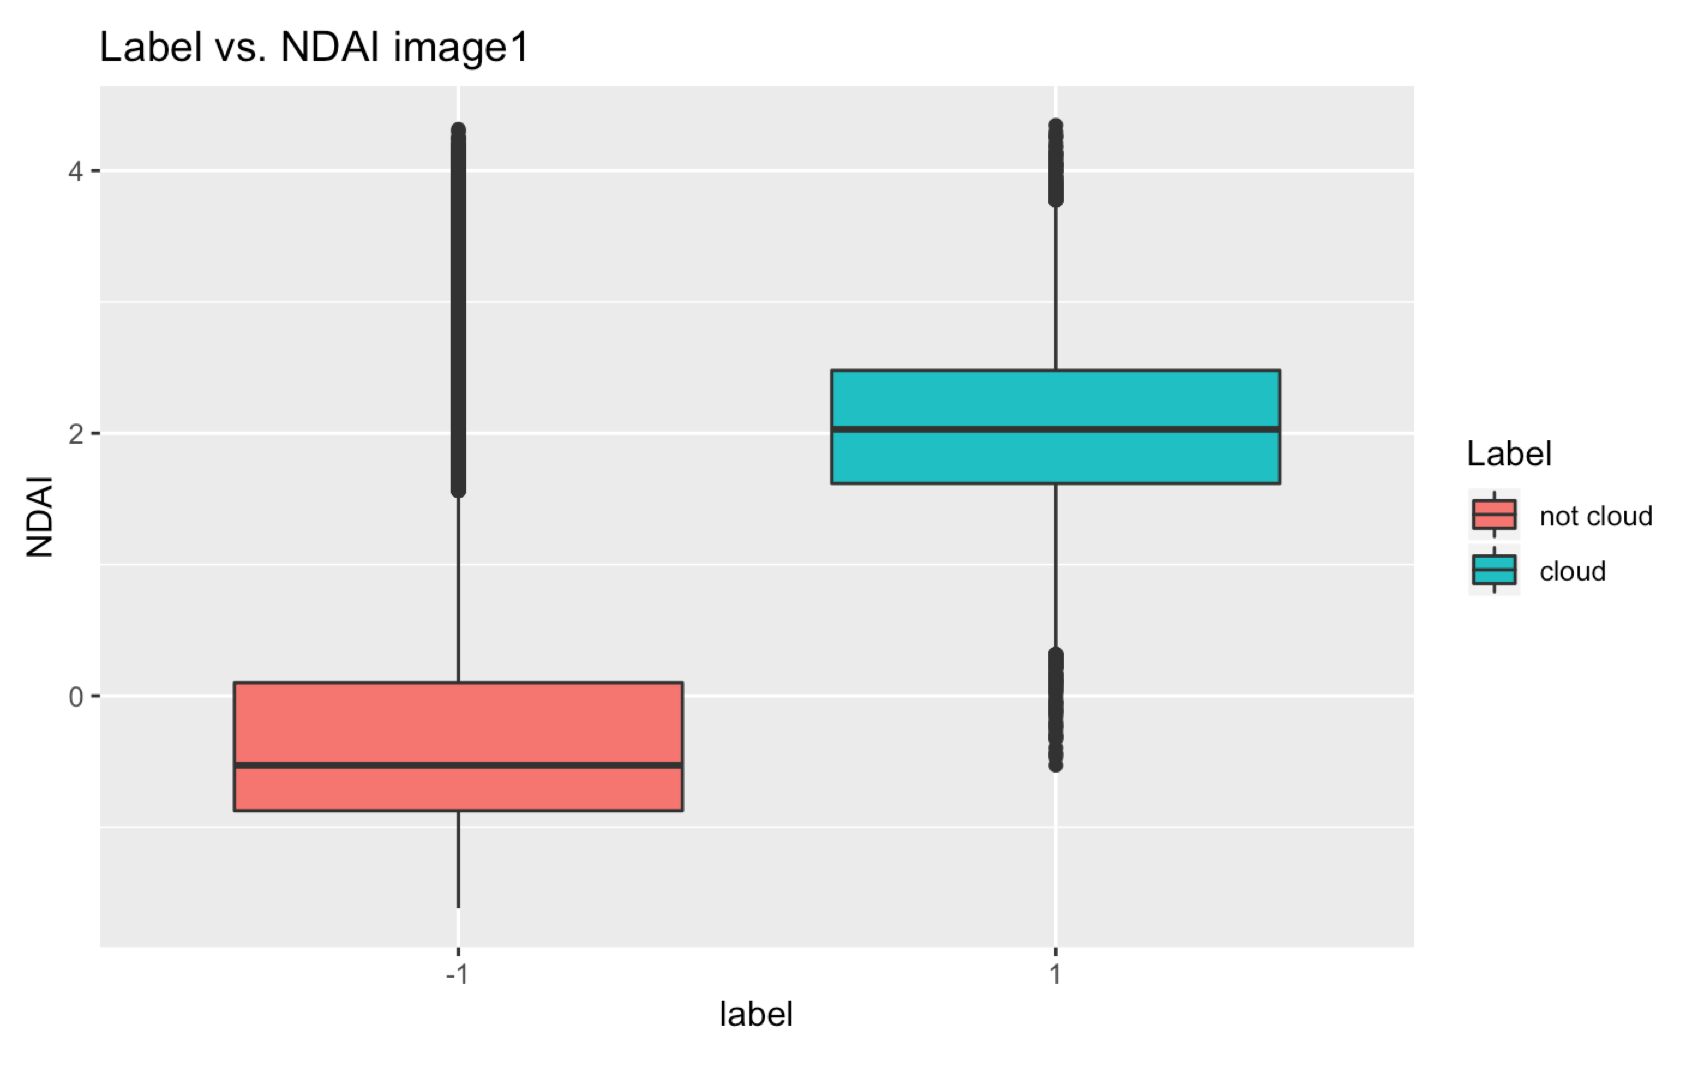
\includegraphics[width = 7.5cm]{1(c)image12.png}
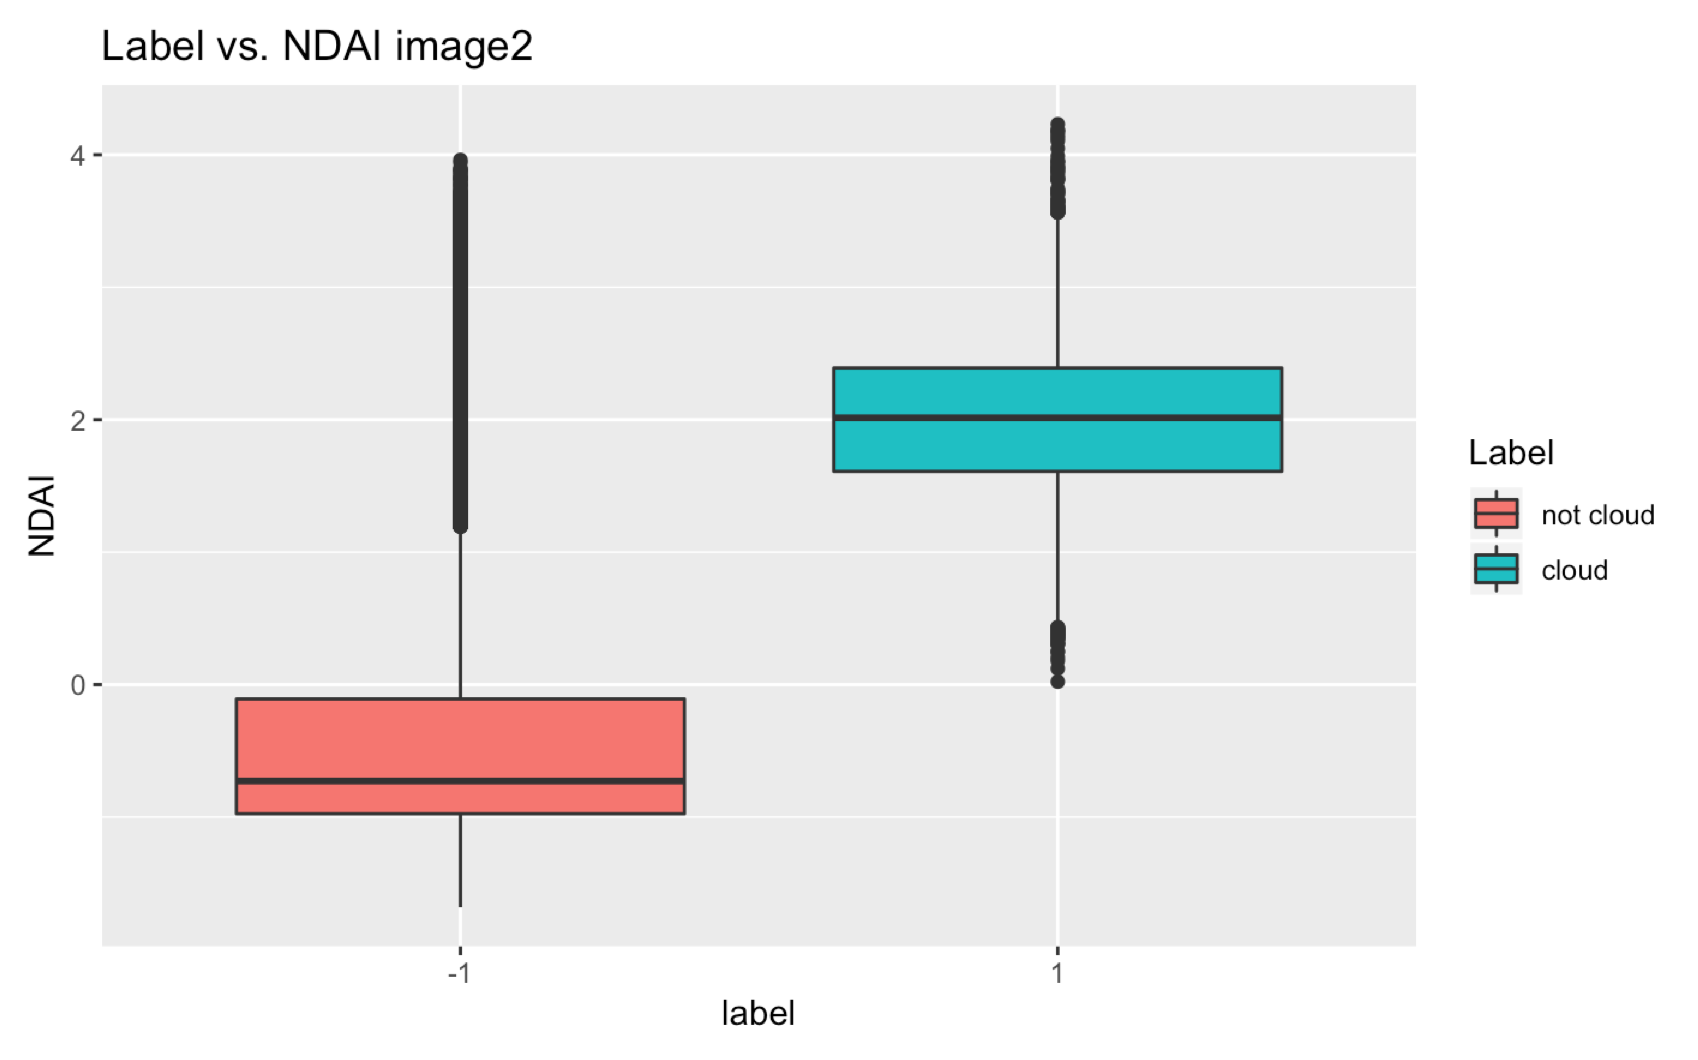
\includegraphics[width = 7.5cm]{1(c)image13.png}

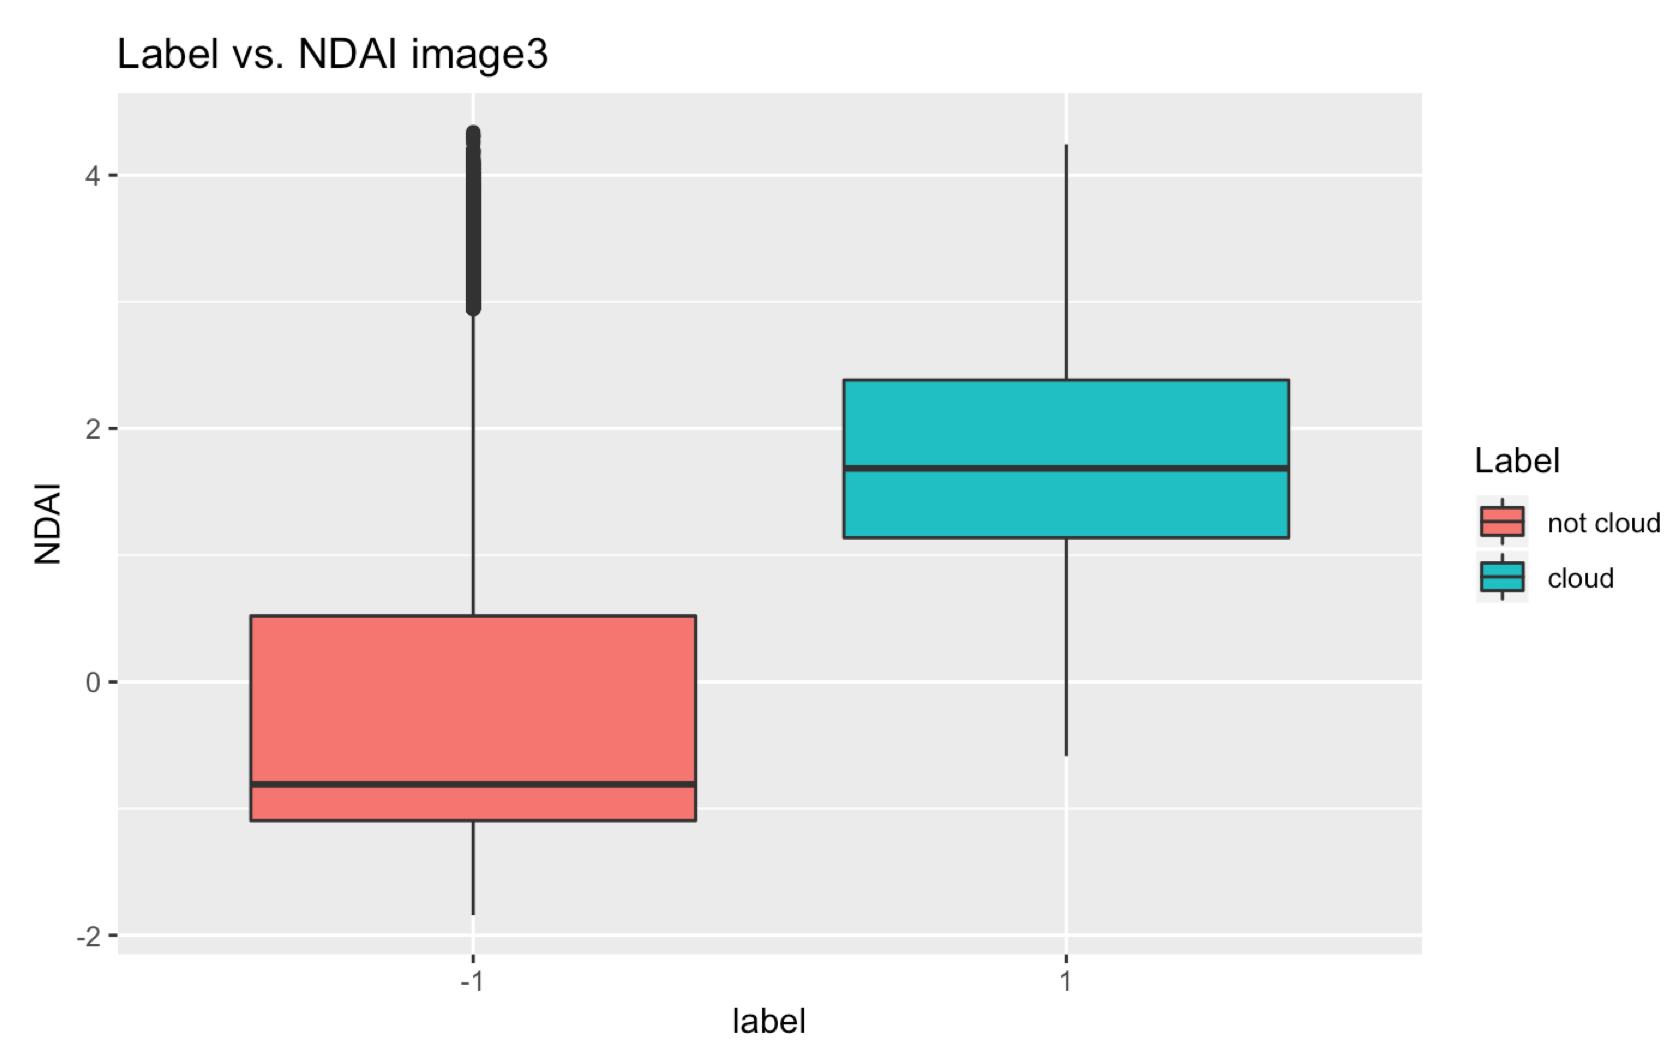
\includegraphics[width = 7.5cm]{1(c)image14.png}
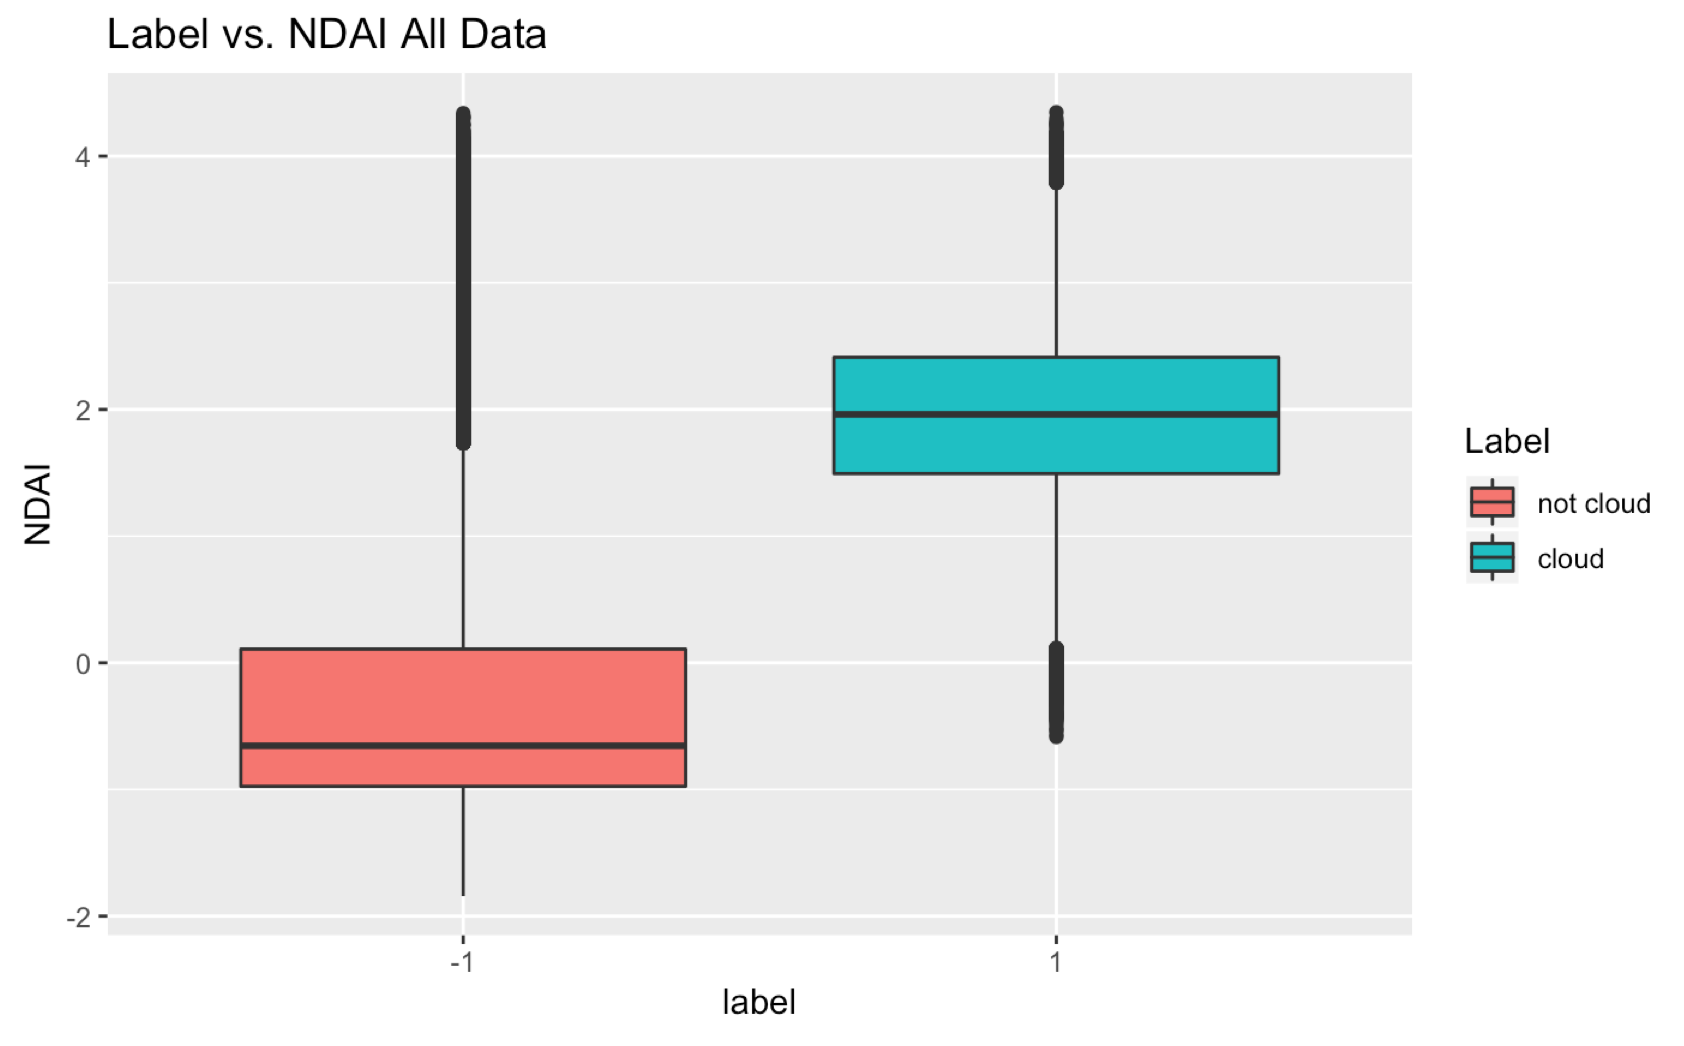
\includegraphics[width = 7.5cm]{1(c)image15.png}

From the boxplots for NDAI based on different labels, we can clearly see that the NDAI is higher for cloud pixels than those cloud-free ones. The distrubition for cloud-free pixels are left skewed, while the distribution for pixels marked as cloud are roughly symmetric. The distribution for three different image data are roughly the same as well.

\section{Preparation}

\vspace{0.2cm}
\textbf{a. Data Split}

Even though the three image data set represent the cloud dsitribution at different times at the same place, we still decide to combine the data into one to have more data for training. We also clear out the unlabeled data here because they are not helpful enough for classification problem. Since the data are not i.i.d., we cannot simply split the data by random. 

First method:
We decided to divide the data into 25 groups by cutting the image horizontally. In this case, data with y\_coord from 2.0-78.2 and the corresponding x-coordinate are in the same group.  We randomly select 23 groups from these 25 groups as training/validation data and 2 groups as test data. In the 23 groups, we randomly sampled 18 groups as validation data. Splitting the data in this way looks like a one-stage cluster sampling. Every time we sample a group wihout replacement and include all data points in that group. Data in the same groups tend to be correlated to each other, which fit the property of the non i.i.d. data.

Our Second method is, for each image data set, to divide all the data into 25 groups by cutting the image into 5*5 small images. For instance, data with y\_coord from 2.0-78.2 and x\_coord from 65.0-125.8 are in the same group. We randomly select 23 groups from these 25 groups as training/validation data and 2 groups as test data. In the 23 groups, we randomly sampled 18 groups as validation data. Splitting the data in this way looks like stratified sampling. Every time we sample a group wihout replacement and include all data points in that group. We can also see this method as combining small pixels into a much larger one in a visual way. This method can guarantee pixels that have high correlations (adjacent pixels) can be sampled at the same time (except those on the boundary). And the random sampling on the 25 groups can make sure that we are not too sticking to the patterns for the training data so that overfitting can be somewhat prevented. 

\vspace{0.3cm}
\mbox{}\\
\textbf{b. Baseline}

Setting all labels to -1, the accuracy for test data is 0.520 and that for validation data is 0.270, which are relatively low. If the test data and validation data contain mostly -1, the trivial classifier will have a high average accuracy.

\vspace{0.3cm}k
\mbox{}\\
\textbf{c. First Order Importance}

To find three best features, we first caculate and plot the correlation between those features and the expert labels. The magnitudes of the absolute values of the correlations represent how close the relationships are between features and expert labels. Larger correlation value means better features. We found that NDAI and CORR are better than others on average. 

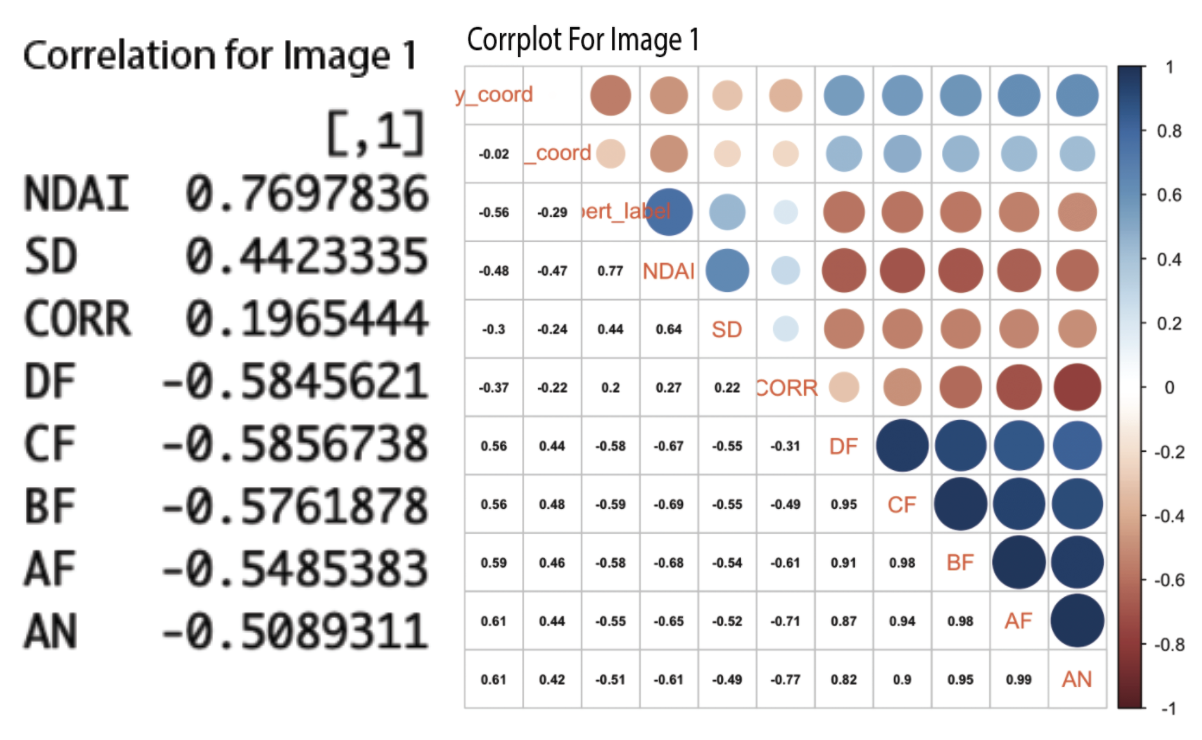
\includegraphics[width = 5.5cm]{2(c)image1.png}
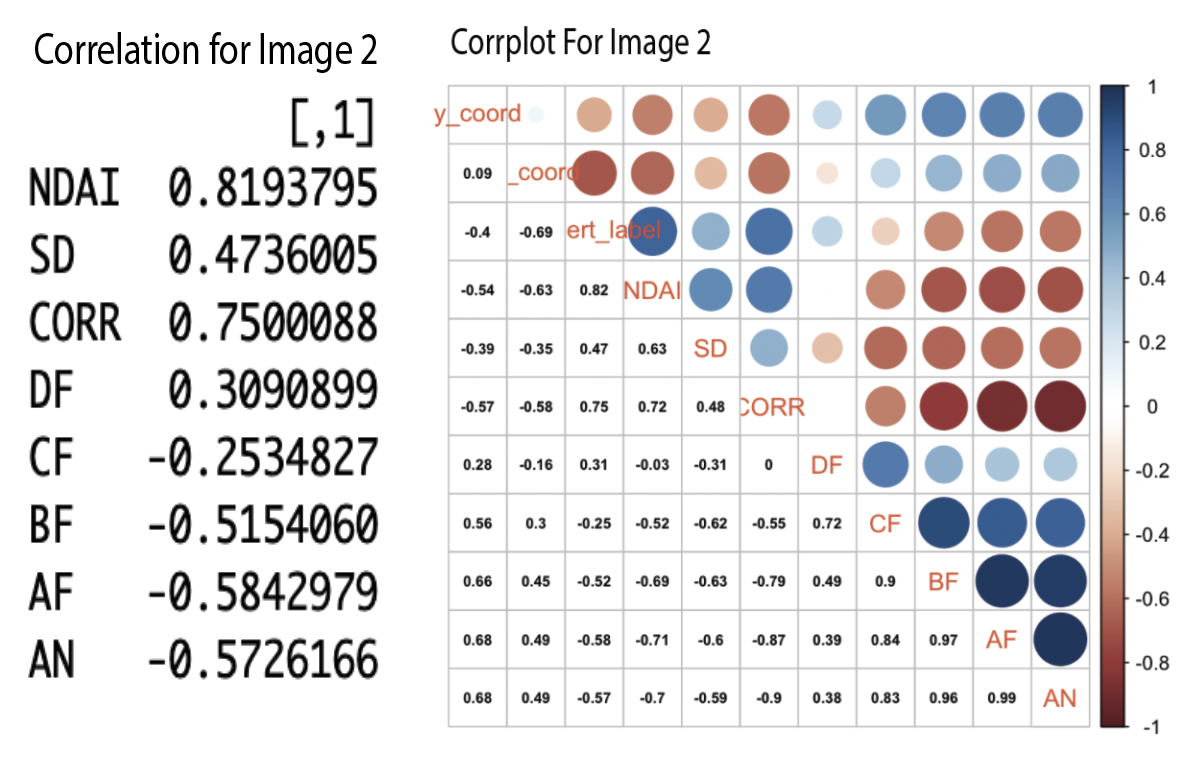
\includegraphics[width = 5.5cm]{2(c)image2.png}
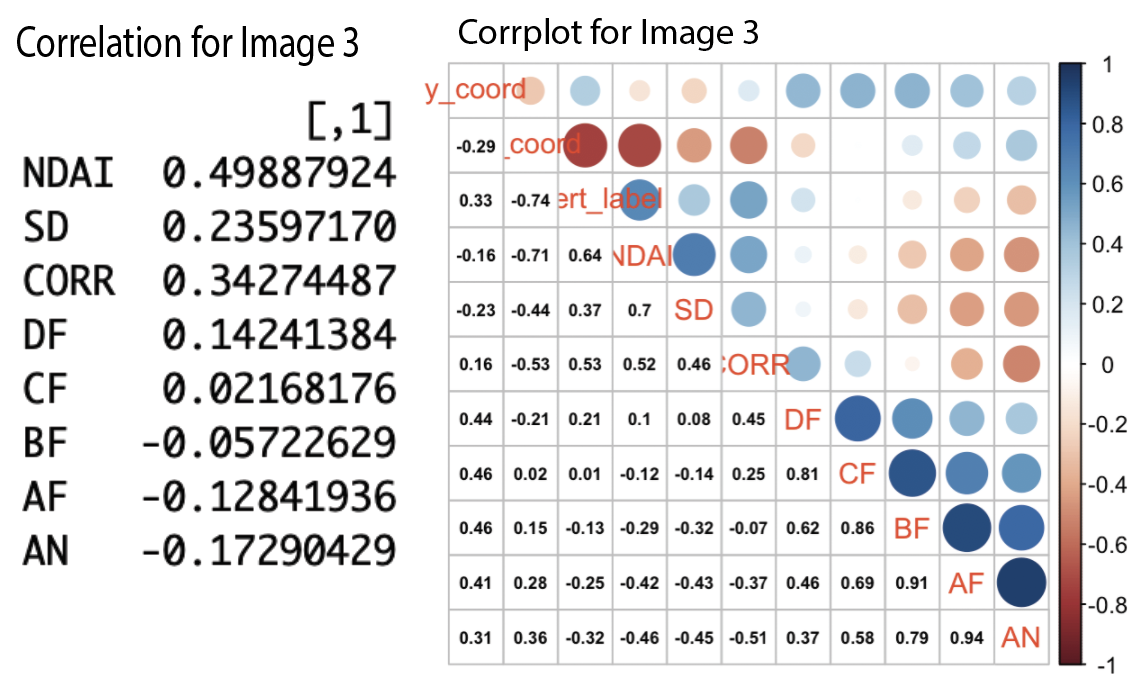
\includegraphics[width = 5.5cm]{2(c)image3.png}

Then, we plot biplots and loadings on first two PCs to see how much each feature contributes to these PCs. We choose to use two PCs because they capture almost 90\% of the data which is enough to represent the entire data set. The loading plots can illustrate the association between features and PCs. The larger the loading of a feature in a given PC, the more associated the feature is with that PC. After viewing the four loading plots, we observe that SD and DF have larger loadings than other features (expect NDAI and CORR). Considering there are other reasons that is more associated with scientific explanation, we decide to be consistent with the three features chosen in the paper, which are CORR, NDAI and SD.




\end{document}
